

\section{Exceptional Events and Environmental Disruptions}
\label{sec:results_exceptional_events_disruptions}

The preceding section characterized recurring population movement under normal-life conditions. The experiments in this section introduce temporary conditions that depart from this reference in two complementary ways. Large-scale events introduce exceptional demand for movement toward specific locations and times, while environmental disruptions change the availability of locations used by the population and may suppress, redirect, or generate additional movement.

Three experiment groups are considered. First, large-scale-event scenarios examine how gathering demand changes population displacement according to event location, the number of concurrent events, and their timing. Second, flood scenarios evaluate how unavailable origins and destinations affect recurring activities and work or school commutes, including the substitution of unavailable activity destinations. Finally, shelter scenarios examine population movement toward capacity-constrained facilities in response to environmental exposure.

Accordingly, this section addresses three main questions: (i) how exceptional gathering demand alters population movement when multiple events occur within the same urban population; (ii) how environmental disruption changes the fulfillment of recurring mobility and what additional burden is introduced by destination adaptation; and (iii) how evacuation demand, shelter capacity, reallocation, and facility disruption affect the protection of exposed populations.


\subsection{Experimental Overview}
\label{sec:exceptional_disruption_overview}

The experiments use the spatial representations introduced in Section~\ref{sec:spatial_representations}. The large-scale-event and shelter experiments use the neighborhood-level environment, whereas the flood-mobility experiments use the reduced and complete census-sector environments. Their durations and outcome measures also differ according to the phenomenon being evaluated. Table~\ref{tbl:exceptional_disruption_scenarios} summarizes the principal comparisons.

\begin{table}[ht]
\centering
\footnotesize
\setlength{\tabcolsep}{4pt}
\caption{Exceptional-event and environmental-disruption experiments and their principal comparisons.}
\label{tbl:exceptional_disruption_scenarios}
\begin{tabularx}{\linewidth}{@{}p{2.9cm}p{3.4cm}p{1.7cm}X@{}}
\toprule
\textbf{Experiment} &
\textbf{Environment} &
\textbf{Duration} &
\textbf{Principal comparison} \\
\midrule

Large-scale events
& Neighborhood-level; 94 regions; population 1,409,351
& 1 day
& No-event baseline and combinations of one to four events are compared to examine event location, concurrent demand, and simultaneous versus staggered execution. \\

Activity disruption
& Reduced and complete census-sector environments
& 56 days
& No exposure is compared with unavailable activity destinations, unavailable homes, and combined exposure to evaluate activity-demand suppression. \\

Flood-aware commuting
& Reduced and complete census-sector environments
& 56 days
& Unavailable homes and destinations are compared to examine their effects on worker and student commute fulfillment. \\

Activity adaptation
& Reduced and complete census-sector environments
& 56 days
& Combined exposure with activity suppression is compared with nearest-available same-type destination substitution. \\

Shelter evacuation
& Neighborhood-level with 104 added shelters; population 1,409,351; mapped exposed population 182,936
& 14 days
& Reallocation, response rate, exposure magnitude, shelter capacity, and selected facility failures are compared. \\

\bottomrule
\end{tabularx}
\end{table}

Because these experiment groups differ in spatial representation, duration, population, and demand definition, their raw outcome quantities are not compared directly across each other. Instead, each set of experiments is evaluated relative to its corresponding reference condition and using the measures appropriate to the simulated process.


\subsection{Large-Scale Events}
\label{sec:results_large_scale_events}

Large-scale events introduce occasional concentrations of population that coexist with the normal-life mobility described in Section~\ref{sec:routine_mobility_neighborhood}. The experiments in this subsection evaluate how these additional demands affect population displacement when the destination, number of concurrent events, and event timing are varied. The gathering mechanism and its configuration are described in Section~\ref{sec:gather_population_plugin_inputs}.

The results correspond to the large-scale-event experiments originally reported with the published manuscript~\cite{silva2026lodusPop}. 
The experiments use the neighborhood-level representation of Porto Alegre, comprising 94 regions, 504 POIs, and a population of 1,409,351. Each simulation covers one 24-hour cycle and uses the neighborhood-level normal-life mobility configuration with a L\'evy scale of 2.

Four event destinations are considered:

\begin{itemize}
    \item Event A: a sports event at the stadium in Farrapos;
    \item Event B: a sports event at the stadium in Praia de Belas;
    \item Event C: a commercial event at the marketplace in Centro Hist\'orico; and
    \item Event D: a cultural event at the university represented by the school POI in Partenon.
\end{itemize}

Figure~\ref{fig:large_event_locations} shows the neighborhoods containing these destinations. Each event requests 500,000 people. This quantity is a scenario-defined stress input rather than an observed attendance value.

\begin{figure}[ht]
    \centering
    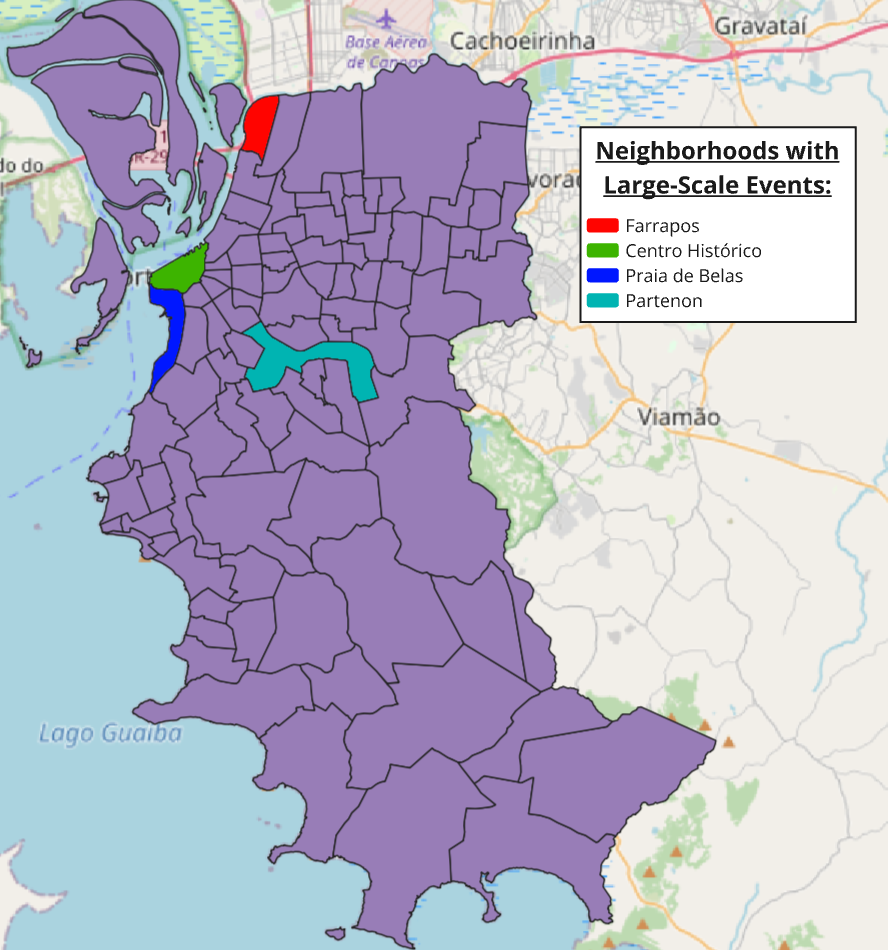
\includegraphics[width=0.70\textwidth]{fig/res-event-disruptions/CityViewNeighborhoods.png}
    \caption{Locations of the four large-scale-event destinations in the neighborhood-level representation of Porto Alegre. Events A and B occur in Farrapos and Praia de Belas, Event C in Centro Hist\'orico, and Event D in Partenon.}
    \label{fig:large_event_locations}
\end{figure}

The experiment configurations contains a no-event baseline and every combination of one, two, three, and four events. 
In these configurations, the selected events occur at 19:00. Because requests scheduled at the same step are processed sequentially, each event operates on the population distribution resulting from the requests processed before it. 
A final configuration uses the same four events but separates part of their demand over the day: Event C occurs at 09:00, Event D at 14:00, and Events A and B at 19:00.

The recorded outcome is population displacement between POIs. One displacement corresponds to one represented person moving from an origin to a destination. %These data characterize the movement generated during the simulation, but they do not separately identify unique event attendees, repeated attendance, fulfilled event demand, or unmet event demand. The results are therefore interpreted in terms of displacement rather than direct event attendance.


\subsubsection{Event Location and Concurrent Demand}
\label{sec:large_event_concurrent_demand}

Table~\ref{tbl:results_displacement} presents the aggregate displacement results for all event configurations. The no-event baseline produces 2,570,658 displacements during the simulated day, corresponding to an average of 1.8240 displacements per inhabitant.

\begin{table}[ht]
\centering
\caption{Displacement results for the large-scale-event simulations. Scenario names identify the events added to the normal-life baseline. All simulations consider the neighborhood-level environment.}
\label{tbl:results_displacement}
\begin{tabular}{@{}lrrr@{}}
\toprule
\textbf{Scenario} &
\shortstack{\textbf{Total}\\\textbf{displacements}} &
\shortstack{\textbf{Displacements}\\\textbf{per inhabitant}} &
\shortstack{\textbf{Increase over}\\\textbf{baseline}} \\
\midrule
Baseline               & 2,570,658 & 1.8240 & --- \\
\midrule
Baseline+A             & 3,290,469 & 2.3347 & 28.00\% \\
Baseline+B             & 3,300,782 & 2.3421 & 28.40\% \\
Baseline+C             & 3,289,002 & 2.3337 & 27.94\% \\
Baseline+D             & 3,281,102 & 2.3281 & 27.64\% \\
\midrule
Baseline+AB            & 3,786,856 & 2.6870 & 47.31\% \\
Baseline+AC            & 3,748,417 & 2.6597 & 45.82\% \\
Baseline+AD            & 3,804,017 & 2.6991 & 47.98\% \\
Baseline+BC            & 3,738,497 & 2.6526 & 45.43\% \\
Baseline+BD            & 3,839,126 & 2.7240 & 49.34\% \\
Baseline+CD            & 3,826,094 & 2.7148 & 48.84\% \\
\midrule
Baseline+ABC           & 4,042,413 & 2.8683 & 57.25\% \\
Baseline+ABD           & 4,109,929 & 2.9162 & 59.88\% \\
Baseline+ACD           & 4,069,223 & 2.8873 & 58.29\% \\
Baseline+BCD           & 4,081,563 & 2.8961 & 58.78\% \\
\midrule
Baseline+ABCD          & 4,235,926 & 3.0056 & 64.78\% \\
Baseline+ABCD+DiffStep & 4,638,329 & 3.2911 & 80.43\% \\
\bottomrule
\end{tabular}
\end{table}

The four single-event configurations produce similar aggregate increases in mobility. Their total displacement ranges from 3,281,102 for Event D to 3,300,782 for Event B, corresponding to increases between 27.64\% and 28.40\% relative to the baseline. Thus, under the same requested event population, the four destinations result in comparable overall movement volumes.

Their spatial distributions, however, are not identical. Figure~\ref{fig:large_event_single_displacement} compares displacement distance for the no-event baseline and each single-event scenario. Although all four events produce similar total displacement, their destinations occupy different parts of the city and consequently draw population over different spatial ranges. For example, Event A produces comparatively more displacement around the longer-distance portion of the distribution. The effect of event location is therefore more visible in the spatial distribution of movement than in its aggregate volume.

\begin{figure}[ht]
    \centering
    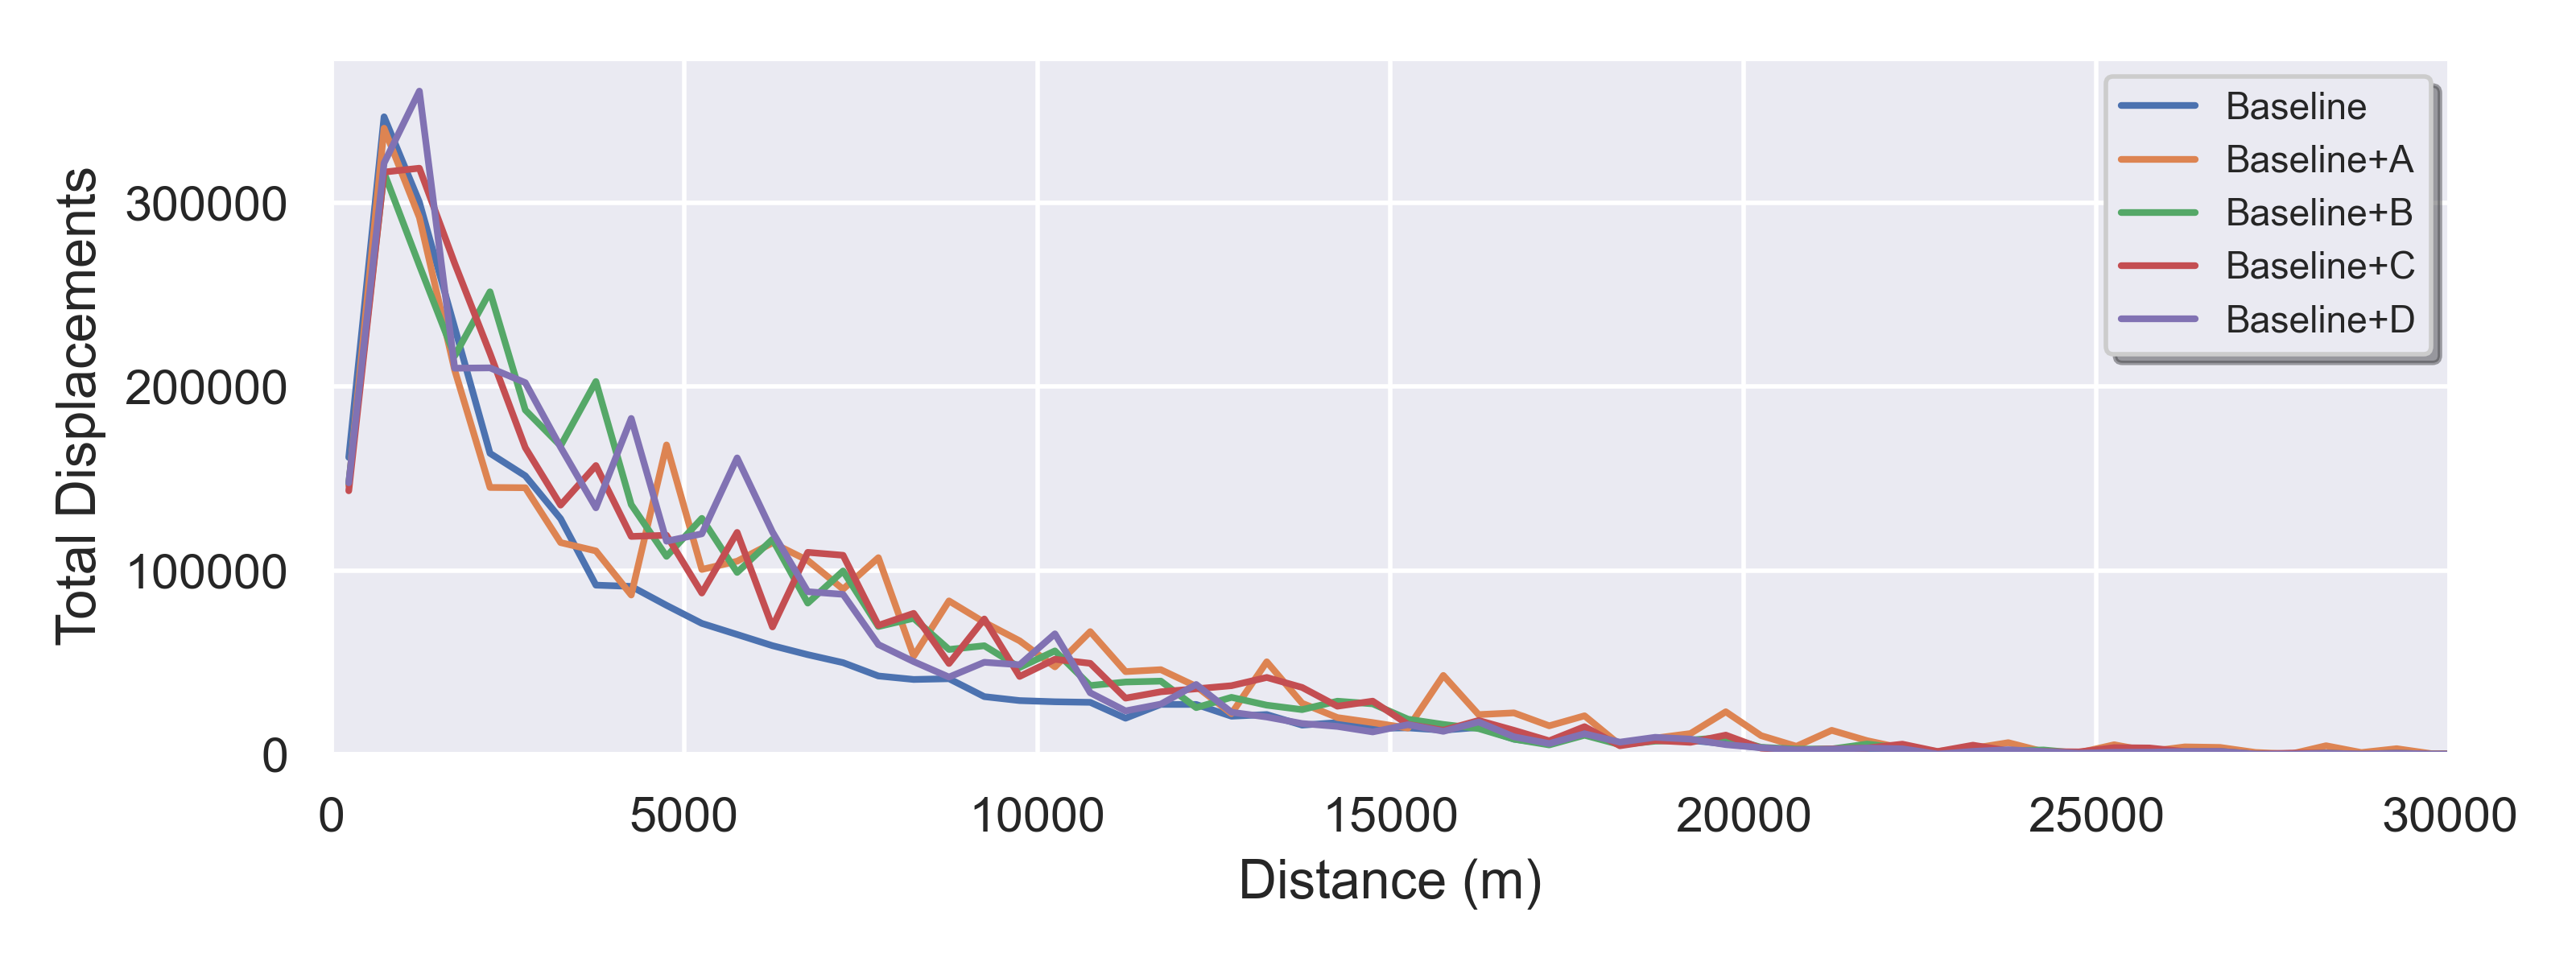
\includegraphics[width=0.98\linewidth]{fig/res-event-disruptions/Displacement_SingleEvent.png}
    \caption{Population-displacement distributions for the no-event baseline and the four single-event scenarios. Each event requests the same population quantity, while differences among the curves reflect the spatial relationship between the event destination and the population available across the city.}
    \label{fig:large_event_single_displacement}
\end{figure}

Adding further simultaneous events progressively increases total displacement. Two-event scenarios produce increases between 45.43\% and 49.34\%, while three-event scenarios produce increases between 57.25\% and 59.88\%. When all four events occur at 19:00, the simulation reaches 4,235,926 displacements, or 64.78\% above the baseline.

However, the effects of concurrent events are not additive. If the events contributed independently to displacement, the combined effect of Events A, B, and C would be expected to approximate the sum of their individual increases. Instead, while Events A, B, and C individually increase displacement by 28.00\%, 28.40\%, and 27.94\%, their simultaneous configuration produces an increase of only 57.25\%. This sub-additive behavior reflects the interaction among event requests operating on the same evolving population state.
%The increase is nevertheless non-additive. For example, Events A, B, and C individually increase displacement by 28.00\%, 28.40\%, and 27.94\%, respectively, whereas their simultaneous ABC configuration increases displacement by 57.25\%. The same pattern is visible as more concurrent events are introduced.

This behavior results from the events operating on the same evolving population state. Population participating in ordinary work and school mobility may already be located away from home when an event request is processed, and each gathering request modifies the population distribution observed by subsequent requests at the same step. Consequently, simultaneous event demands cannot be interpreted as independent additions to the normal-life baseline.

The resulting non-additivity is evidence of interaction among concurrent population demands, but it should not be interpreted as a direct measurement of event-attendance fulfillment. The preserved results do not record the requested and fulfilled attendance of each event separately.


\subsubsection{Event Timing}
\label{sec:large_event_timing}

The final comparison examines how the timing of Events A, B, C, and D affects population displacement, comparing a configuration in which all four events occur simultaneously with one in which their demands are distributed throughout the day.
%The final comparison examines the temporal distribution of the same four event demands. 
Figure~\ref{fig:large_event_timing_displacement} compares the baseline with the four-event simultaneous configuration and the condition in which Events C and D occur earlier in the day.

\begin{figure}[ht]
    \centering
    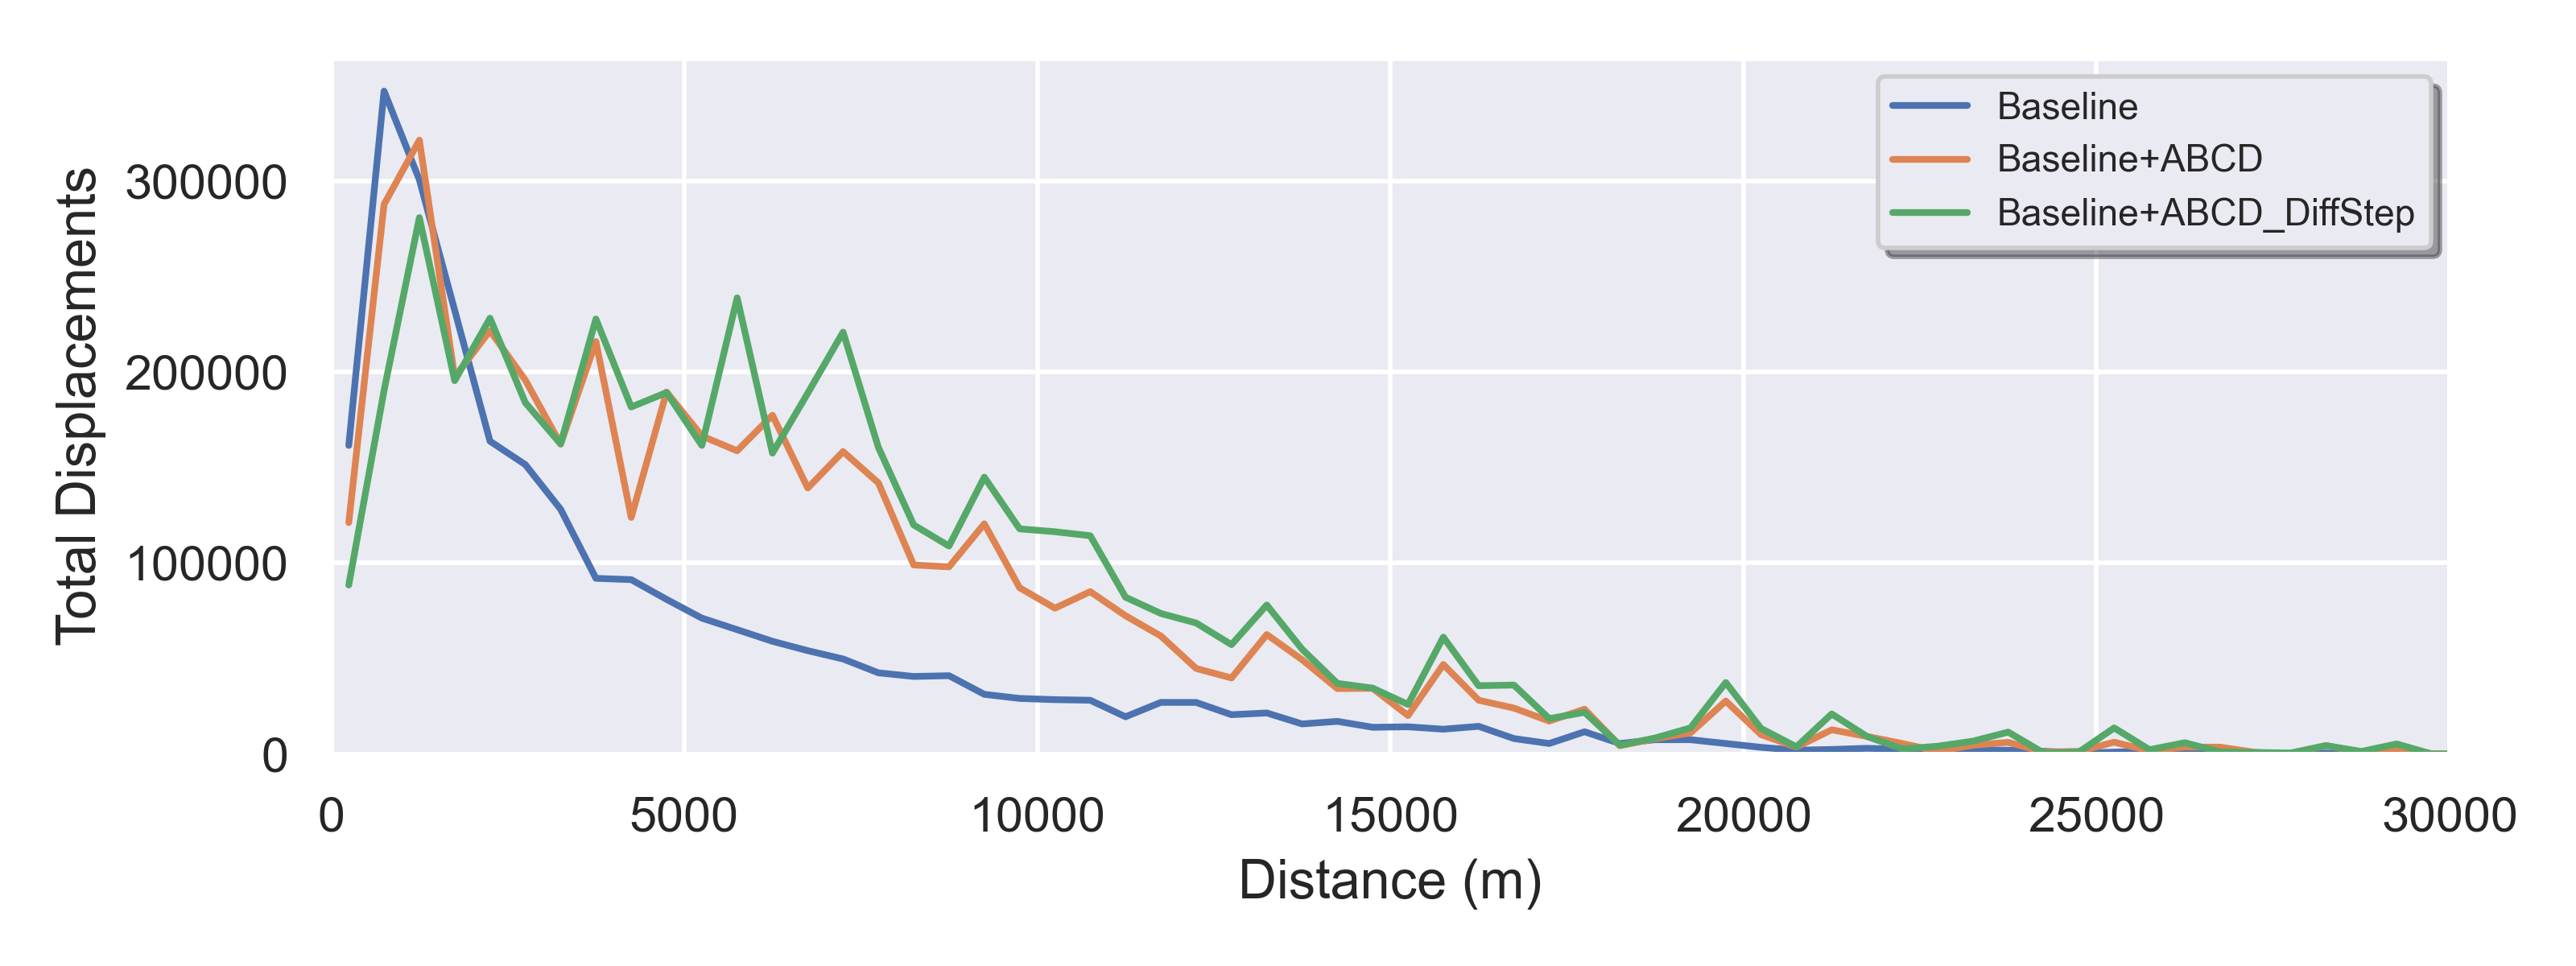
\includegraphics[width=0.98\linewidth]{fig/res-event-disruptions/Displacement_AllEvents.png}
    \caption{Population-displacement distributions for the no-event baseline, four events occurring simultaneously at 19:00, and the staggered four-event configuration in which Event C occurs at 09:00, Event D at 14:00, and Events A and B at 19:00.}
    \label{fig:large_event_timing_displacement}
\end{figure}

With all four events occurring simultaneously, total displacement reaches 4,235,926, corresponding to 3.0056 displacements per inhabitant and an increase of 64.78\% over the no-event baseline. When Events C and D occur earlier, total displacement increases to 4,638,329, or 3.2911 displacements per inhabitant. This represents an 80.43\% increase over baseline and 402,403 additional displacements relative to the simultaneous four-event configuration.

The difference shows that exceptional demand is affected by when it is introduced, not only by its total requested quantity. When four requests are concentrated at the same step, they operate sequentially on the population available at that moment. Separating part of this demand over the day allows the population distribution to evolve between requests, so population relocated earlier may subsequently become available for other movements or later gathering requests.

Overall, the large-scale-event experiments show that exceptional gathering demand affects both the volume and spatial distribution of population mobility. Event destinations with the same requested population produce similar aggregate displacement but different distance distributions. Increasing the number of simultaneous events raises total movement, although the resulting effect is not additive because the requests interact through a shared and changing population state. Finally, distributing the same four event demands over different times produces more displacement than concentrating them at a single simulation step. These results establish the effects of exceptional demand before the following experiments consider a different departure from normal-life mobility: environmental conditions that make locations temporarily unavailable.


\subsection{Flood-Induced Mobility Disruption}
\label{sec:results_flood_mobility}

The large-scale-event experiments introduce additional demand while leaving the underlying environment available. Flooding produces a different departure from normal-life mobility by making some of the locations used by recurring activities and commutes temporarily unavailable. The experiments in this subsection examine how this disruption affects activity visits and work or school attendance, and whether activity demand can be preserved by redirecting visits toward alternative destinations.

The experiments use the reduced and complete census-sector environments introduced in Section~\ref{sec:census_sector_environments}. The reduced environment comprises 13 regions, 2,610 POIs, and a population of 159,886, while the complete environment comprises 94 regions, 16,266 POIs, and a population of 1,331,414. Each simulation covers 56 days with 24 hourly steps per day and applies the time-varying water-level series described in Section~\ref{sec:water_level_plugin_inputs}.

Three types of comparisons are considered. First, activity scenarios expose homes, activity destinations, or both to flooding and measure the resulting fulfillment of visits to marketplaces, restaurants, and pharmacies. Second, attendance-controlled commute scenarios additionally expose work and school destinations, allowing the effects on recurring work and school mobility to be measured. Finally, an adaptation scenario allows unavailable activity destinations to be replaced by the nearest available POI of the same type. Work and school destinations remain non-substitutable under the evaluated configuration.


\subsubsection{Environmental Exposure and Mobility Loss}
\label{sec:flood_environmental_exposure}

The applied water-level series changes the number and spatial distribution of POIs available throughout the 56-day simulation. Figure~\ref{fig:environment_disruption_flood_exposure} presents the simulated water-level sequence together with the POI availability state at its maximum value of 5.33~m.

At this maximum level, 513 of the 2,610 POIs in the reduced environment and 1,920 of the 16,266 POIs in the complete environment are unavailable. The affected locations include homes, activity destinations, workplaces, and schools, creating periods in which recurring mobility can no longer be executed under the same conditions as the normal-life baseline.

%SO: acrescentei abaixo
%GA: certo
As a plausibility reference, the maximum water level considered in this experiment (5.33 m) corresponds to the historical peak reported for the Guaíba during the May 2024 flood, reached on May 5 and 6. During this event, 157,701 people were reported as affected in Porto Alegre, corresponding to 11.8\% of the city’s population.\footnote{CNN Brasil, “Enchente afetou quase 12\% da população de Porto Alegre; veja números sobre o impacto da chuva na cidade,” May 16, 2024. Available at: \url{https://www.cnnbrasil.com.br/nacional/enchente-afetou-quase-12-da-populacao-de-porto-alegre-veja-numeros-sobre-o-impacto-da-chuva-na-cidade/}}. At the same maximum water level, 1,920 of the 16,266 POIs in the complete simulated environment are unavailable, also corresponding to approximately 11.8\%. Although the percentage of unavailable POIs and the percentage of affected population represent different quantities and are therefore not directly comparable, their similar order of magnitude provides a useful contextual reference for the scale of environmental exposure represented in the experiment. This comparison is intended as a plausibility reference rather than as an empirical validation of the simulated flood impacts.


\begin{figure}[ht]
    \centering
    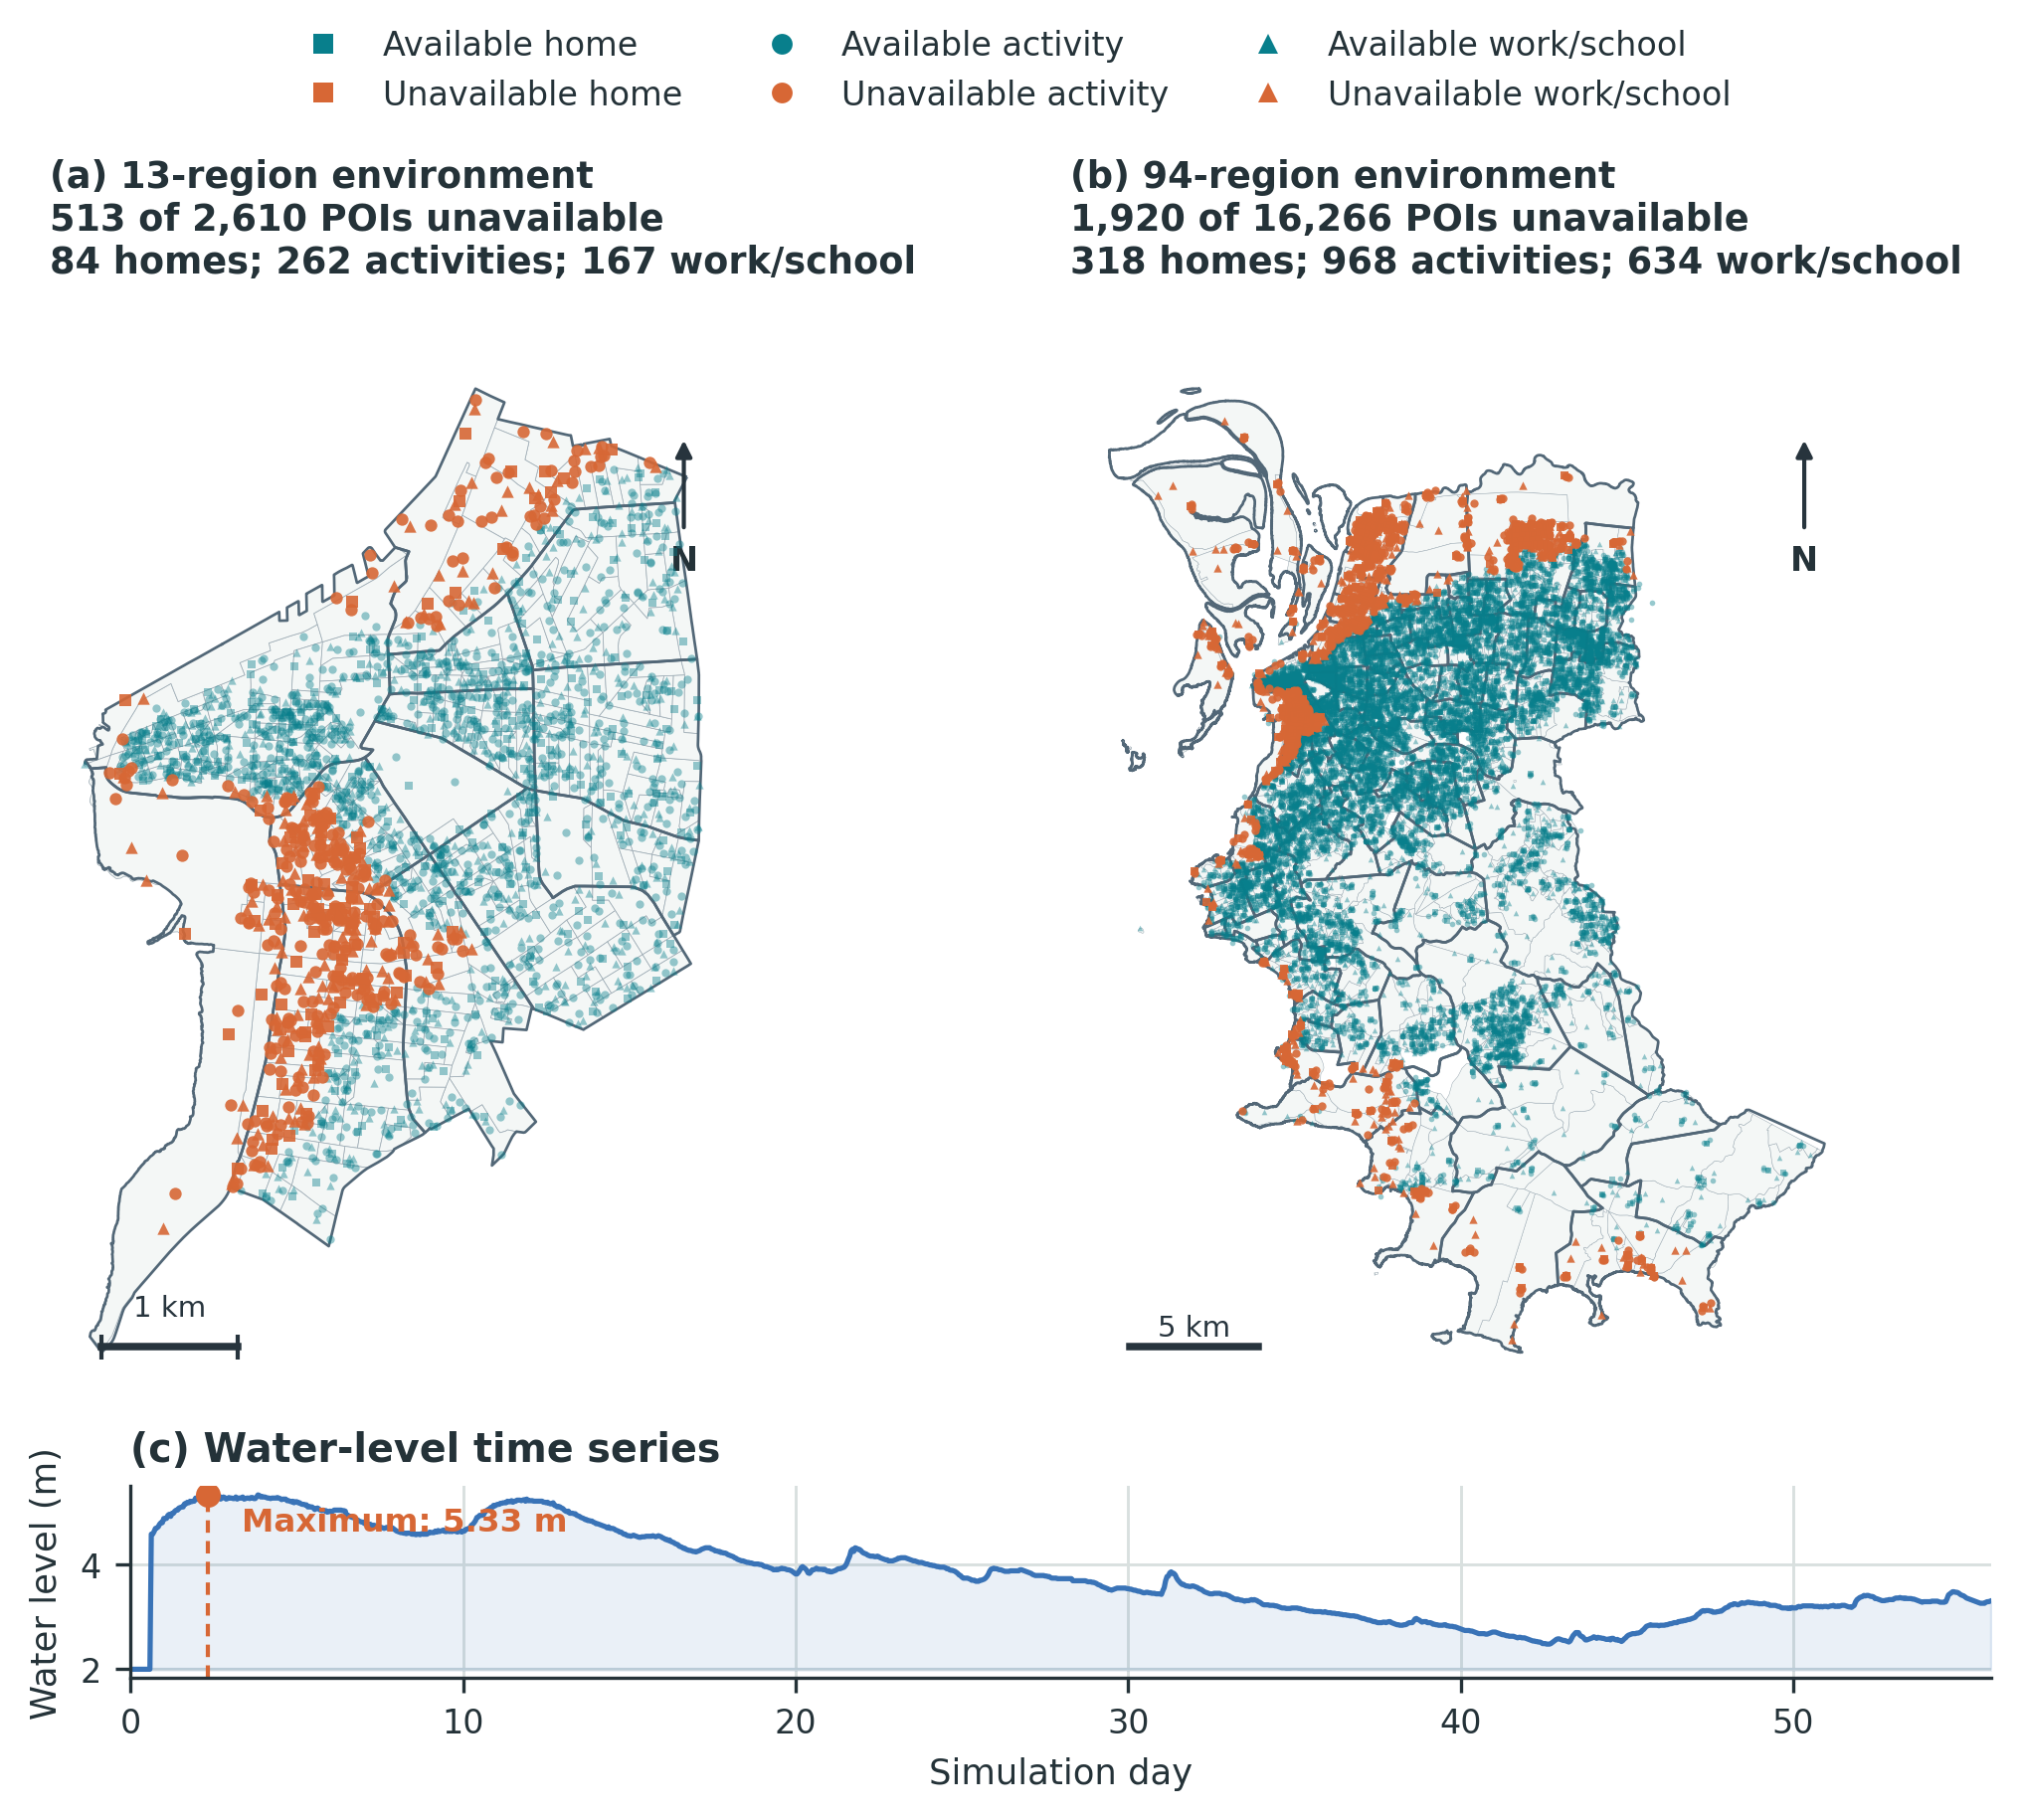
\includegraphics[width=\linewidth]{fig/res-event-disruptions/environment_disruption_flood_exposure.png}
    \caption{POI availability under the simulated flood conditions. Panels (a) and (b) show available and unavailable POIs at the maximum simulated water level of 5.33~m in the reduced and complete census-sector environments, respectively. Panel (c) presents the water-level series applied throughout the 56-day simulation.}
    \label{fig:environment_disruption_flood_exposure}
\end{figure}

The resulting mobility loss depends on whether flooding affects an origin or a requested destination. Figure~\ref{fig:flood_fulfillment_comparison} summarizes activity and commute fulfillment under the different exposure conditions.

%GA: poderia ser uma tabela. Se manter figura, ajustar o inicio do eixo X
\begin{figure}[ht]
    \centering
    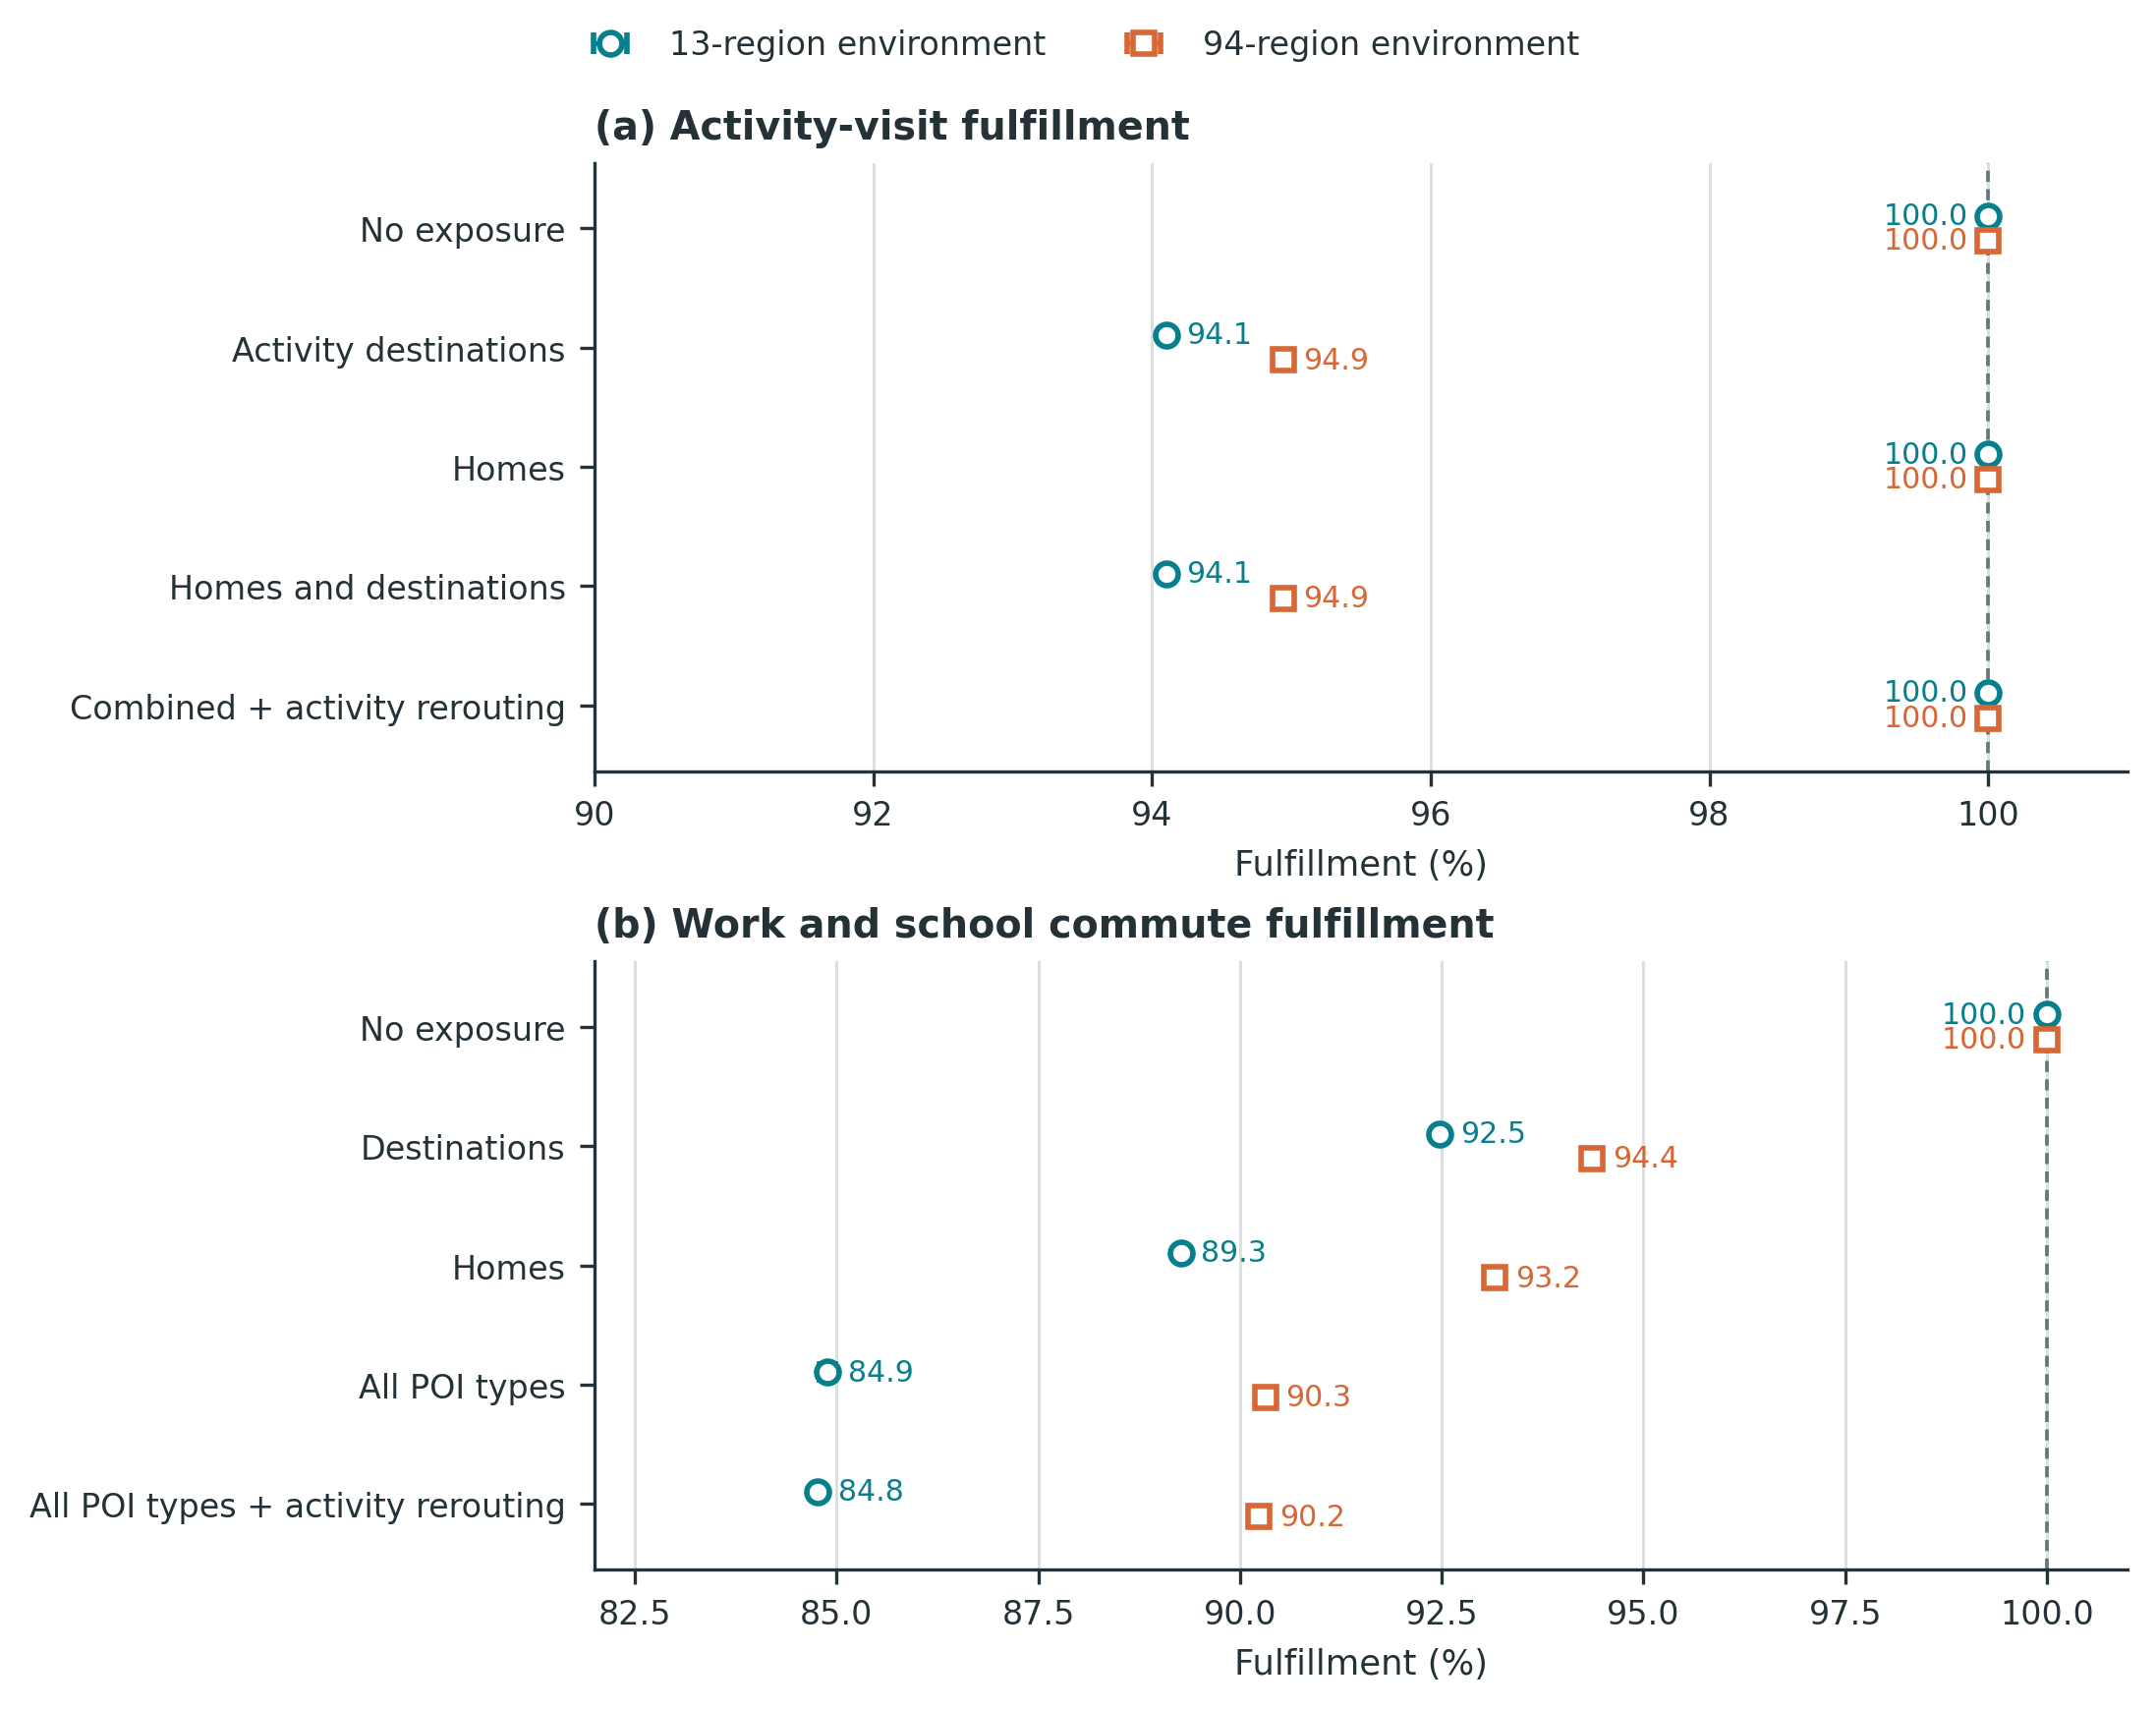
\includegraphics[width=\linewidth]{fig/res-event-disruptions/environment_disruption_fulfillment_comparison.png}
    \caption{Mobility fulfillment under the evaluated flood conditions in the reduced and complete census-sector environments. Panel (a) shows activity-visit fulfillment and panel (b) shows the combined fulfillment of work and school commutes. Results compare the normal-life reference with unavailable destinations, unavailable homes, combined exposure, and combined exposure with activity-destination substitution. Points are means over five simulation runs.}
    \label{fig:flood_fulfillment_comparison}
\end{figure}

For activity visits, unavailable destinations are the main source of lost demand. In the reduced environment, activity fulfillment decreases from 100\% under the reference condition to 94.10\% when marketplaces, restaurants, and pharmacies are exposed, corresponding to 169,736 unmet visits over the 56-day simulation. Exposing homes alone does not reduce activity fulfillment, and exposing homes and destinations together produces the same 94.10\% fulfillment as destination exposure alone.

The complete environment presents the same general pattern. Activity-destination exposure reduces fulfillment from approximately 100\% to 94.94\%, leaving approximately 1.21 million visits unmet. Home exposure alone has negligible effect on the number of fulfilled visits, while combined home and destination exposure again produces approximately the same activity loss as destination exposure.

These results indicate that the activity configuration can compensate for unavailable population sources by drawing eligible population from other available homes. It cannot, however, complete a requested visit when its activity destination is unavailable unless destination substitution is enabled.

Work and school commutes are affected differently because both the population origin and the requested destination are required for attendance. In the reduced environment, commute fulfillment decreases from effectively 100\% under normal-life conditions to 92.47\% when destinations are exposed and to 89.27\% when homes are exposed. When all relevant POI types are exposed, fulfillment falls further to 84.89\%.

The same pattern occurs in the complete environment, although the reduction is smaller. Destination exposure results in 94.36\% commute fulfillment, home exposure in 93.16\%, and combined exposure in 90.31\%. Thus, flooding both origins and destinations produces the largest disruption in both spatial representations.

Under combined exposure, student fulfillment remains slightly higher than worker fulfillment. In the reduced environment, the respective means are 86.30\% and 84.33\%, a difference of 1.96 percentage points. In the complete environment, the respective means are 90.66\% and 90.18\%, a difference of 0.49 percentage points. %Because this separation is modest, particularly in the complete environment, Figure~\ref{fig:flood_fulfillment_comparison} retains the aggregate commute result.

Unlike the activity results, where unavailable homes can largely be compensated by alternative population sources, commute demand is tied to the population's home and requested work or school destination. As a result, unavailable origins as well as unavailable destinations contribute directly to unmet attendance.

Completed-trip distance is not emphasized as a primary disruption measure. In several flooded conditions, the mean distance among completed movements decreases because some trips are suppressed entirely. Such changes therefore describe the subset of movements that remain feasible rather than an improvement in accessibility.


\subsubsection{Activity-Destination Adaptation}
\label{sec:flood_destination_adaptation}

The final flood-mobility comparison examines whether activity demand lost through unavailable destinations can instead be redirected toward alternative locations. Under this configuration, a visit whose requested marketplace, restaurant, or pharmacy is unavailable is assigned to the nearest available POI of the same type. The requested and receiving destinations remain distinguishable in the results, allowing the amount of recovered demand and the additional spatial burden of substitution to be measured. %GA: burden foi o termo sugerido para "carga" adicional (população extra que os POIs recebem quando demanda é redirecionada)

In the reduced environment, substitution restores all 169,736 activity visits that would otherwise be suppressed by destination unavailability. In the complete environment, it restores essentially all of the approximately 1.21 million affected visits, leaving only about five unmet requests per run. Activity fulfillment therefore returns to approximately 100\% in both environments.

This recovery is accompanied by additional displacement between the requested and receiving destinations. Rerouted visits travel an average of approximately 294~m beyond their requested destination in the reduced environment and 1.17~km in the complete environment. Figure~\ref{fig:flood_rerouting_burden} summarizes this trade-off together with the redistribution of demand among receiving POIs.

%GA: também poderia ser uma tabela
\begin{figure}[ht]
    \centering
    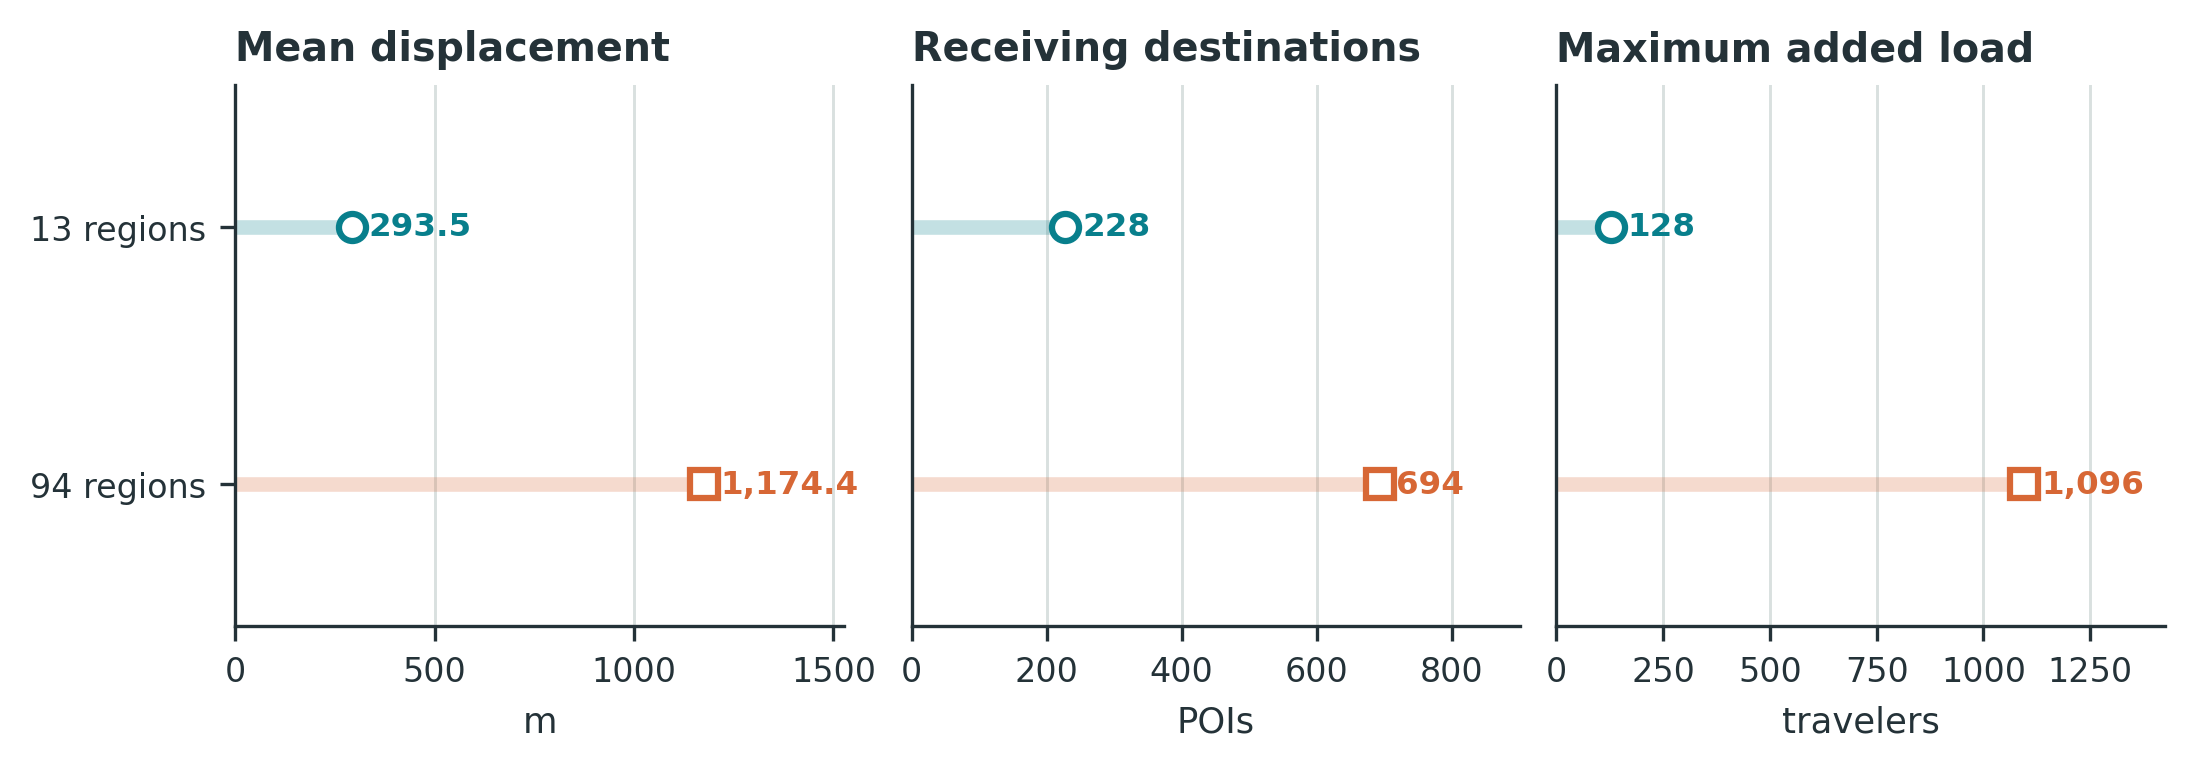
\includegraphics[width=\linewidth]{fig/res-event-disruptions/environment_disruption_rerouting_burden.png}
    \caption{Activity-destination adaptation under combined home and destination exposure to flood. The panel on the left shows the mean displacement between requested and receiving destinations, the panel in the center shows the number of distinct receiving activity POIs, and the panel on the right shows the peak rerouted-only concurrent population at one receiving POI, excluding direct demand. Values are means over five simulation runs for the reduced and complete census-sector environments.}
    \label{fig:flood_rerouting_burden}
\end{figure}

%SO: re-escrevi porque achei confuso, e acho que falta o total -- 228 de quantas???
%GA: adicionei os totais
Under the activity-destination substitution configuration, the demand redirected from unavailable destinations is distributed among 228 of the 1,305 activity POIs in the reduced environment and 694 of the 8,133 in the complete environment.
%The redirected demand is distributed among 228 receiving activity POIs in the reduced environment and 694 in the complete environment. 
The largest additional concurrent concentration attributable to rerouted population reaches 128 people at one receiving POI in the reduced environment and 1,096 in the complete environment.

These values do not represent facility-capacity violations, since activity destinations are not assigned service capacities in this experiment. Instead, they characterize how the nearest-available substitution policy redistributes demand when the originally requested locations cannot be used. The complete environment requires substantially greater displacement and produces larger concentrations of redirected population under the same adaptation rule.

Importantly, this adaptation applies only to activity destinations. Workplaces and schools remain associated with their originally requested destinations. Consequently, restoring activity demand does not restore commute fulfillment. Under combined exposure, commute fulfillment remains approximately 84.8\% in the reduced environment and 90.2\% in the complete environment whether activity substitution is enabled or not.

The flood experiments therefore show two distinct responses to unavailable urban locations. Without adaptation, flooding suppresses recurring movement, with the largest commute losses occurring when both origins and destinations are affected. Allowing substitution can preserve almost all activity demand, but transfers part of the disruption into additional travel and greater demand at alternative destinations. Work and school attendance remains constrained because these destinations are not treated as interchangeable.

These results provide a complementary view of exceptional mobility to the large-scale-event experiments. Large-scale events add demand to an otherwise available environment, whereas flooding removes some of the locations required by normal-life movement. The shelter experiments considered next extend this disruption further by introducing new protection-seeking movement toward a capacity-constrained network of facilities.


\subsection{Evacuation and Shelter Response}
\label{sec:results_shelter_response}

The preceding experiments examined two departures from normal-life mobility: large-scale events, which introduce additional movement toward exceptional destinations, and flooding, which disrupts recurring activities and commutes by making some locations temporarily unavailable. 
Environmental disruptions may also generate new movement in response to population exposure. The shelter experiments examine this additional response by representing populations affected by flooding and evaluating their relocation toward a spatially distributed and capacity-constrained shelter network.

The experiments use the neighborhood-level environment, comprising 94 regions, 504 base POIs, and a population of 1,409,351. 
The 104 shelter POIs described in Section~\ref{sec:shelter_plugin_inputs} are added to this environment, resulting in 608 POIs. These POIs are derived from the recorded locations and capacities of shelters operating in Porto Alegre on May 15, 2024, using the real-world data source documented in that section
%SO: talvez fosse legal citar que tiveram a ver com as localizações reais dos shelters
%GA: a section de shelter já indica que são dados reais, mas também ajustei aqui.
The resulting shelter network provides a total recorded capacity of 12,519 people and has a configured initial occupancy of 10,963.
Population exposure is based on a fixed 5.30~m flood condition. After mapping the exposure data to the represented population, 182,936 people are classified as exposed and constitute the reference population used in the shelter analysis.

Each experiment covers 14 simulated days with 24 hourly steps per day. Under the reference configuration, 1\% of the exposed population is requested to evacuate per day. Evacuation requests occur at 07:00, admission to shelters is evaluated at 08:00, optional waitlist reallocation occurs at 09:00, and populations moved during reallocation are reconsidered for admission at 10:00.

The evaluated scenarios vary five aspects of this reference configuration: waitlist reallocation, daily response rate, exposure magnitude, shelter capacity, and shelter availability. Table~\ref{tbl:shelter_scenarios} summarizes the corresponding scenario groups. Each configuration is evaluated over five simulation runs. Reported values are means across these runs.%; variability is generally small and is shown in the corresponding figures where applicable.

\begin{table}[ht]
\centering
\footnotesize
\caption{Shelter scenarios and their principal comparisons.}
\label{tbl:shelter_scenarios}
\begin{tabularx}{\linewidth}{@{}p{3.1cm}p{3.0cm}X@{}}
\toprule
\textbf{Scenario group} &
\textbf{Configurations} &
\textbf{Principal comparison} \\
\midrule

Reallocation
& Off; on
& Whether redistributing waiting populations reduces congestion or improves the use of remaining shelter capacity. \\

Daily response rate
& 0.5\%, 1\%, 2\%, 5\%
& Whether introducing evacuation demand more rapidly increases protection or primarily increases congestion. \\

Exposure magnitude
& 0.25$\times$, 0.5$\times$, 1$\times$
& How changes in exposed population affect unresolved demand under fixed shelter capacity. \\

Shelter capacity
& 0.5$\times$, 1$\times$, 2$\times$, 5$\times$, 15$\times$
& At what point increasing accommodation ceases to improve protection within the 14-day simulation. \\

Shelter failure
& Largest shelter disabled; highest-capacity shelters disabled
& How loss of accommodation affects protection and whether reallocation mitigates the resulting congestion. \\

\bottomrule
\end{tabularx}
\end{table}

The analysis distinguishes final protection from congestion. Shelter coverage is defined as the final population with a \texttt{sheltered} status divided by the 182,936 mapped exposed population. Because this value includes the configured initial occupancy, it should not be interpreted as the number of people newly admitted during the simulation. Unresolved demand corresponds to the population remaining in the \texttt{in\_danger} state, while peak waitlist and accumulated waiting-person-hours characterize congestion.

Under the reference configuration, 1,556 people are newly admitted after the simulation begins. Together with the initial occupancy of 10,963, this produces a final sheltered population of 12,519, equal to the available reference capacity. Distinguishing these quantities is important: final coverage describes the shelter occupancy achieved at the end of the scenario, whereas new admissions describe the additional protection provided during the simulated evacuation period.


\subsubsection{Reference Evacuation and Reallocation}
\label{sec:shelter_reference_reallocation}

The reference experiment establishes how evacuation demand develops under the recorded shelter capacity. Table~\ref{tbl:shelter_reference_results} compares the same scenario with waitlist reallocation disabled and enabled. Accumulated waiting last column in the table) is measured in person-hours and corresponds to the sum, over all simulation steps, of the population waiting for shelter admission. For example, 1,000 people remaining on a waitlist for 10 hours contribute 10,000 person-hours of accumulated waiting. Values are reported in millions of person-hours for readability.

\begin{table}[ht]
\centering
\footnotesize
\caption{Mean shelter outcomes over five simulation runs under the reference configuration.}
\label{tbl:shelter_reference_results}
\begin{tabular}{@{}lrrrr@{}}
\toprule
\textbf{Policy} &
\shortstack{\textbf{Coverage}\\\textbf{(\%)}} &
\shortstack{\textbf{Unresolved}\\\textbf{demand}} &
\shortstack{\textbf{Peak}\\\textbf{waitlist}} &
\shortstack{\textbf{Waiting}\\\textbf{(million person-h)}} \\
\midrule
No reallocation
    & 6.843 & 170,417 & 24,195 & 3.998 \\
Reallocation
    & 6.843 & 170,417 & 24,195 & 3.950 \\
\bottomrule
\end{tabular}
\end{table}

At the end of both conditions, all 12,519 shelter places are occupied, corresponding to 6.843\% of the mapped exposed population. The remaining 170,417 people retain an \texttt{in\_danger} status. Reallocation therefore does not increase final protection when the network is already capacity constrained.
It does, however, reduce accumulated waiting. Across the 14-day simulation, reallocation lowers waiting by approximately 48,000 person-hours, or 1.2\%. %The associated change in travel distance is small, with mean distance increasing by approximately 0.03~km as some waiting populations are redirected toward alternative shelters.

Figure~\ref{fig:shelter_reference_dynamics} shows how this behavior develops over time. Under the reference configuration, the shelter network reaches its full available capacity after approximately 32 simulated hours. Additional evacuation requests thereafter cannot increase the sheltered population and instead contribute primarily to unresolved demand and waiting.

\begin{figure}[ht]
    \centering
    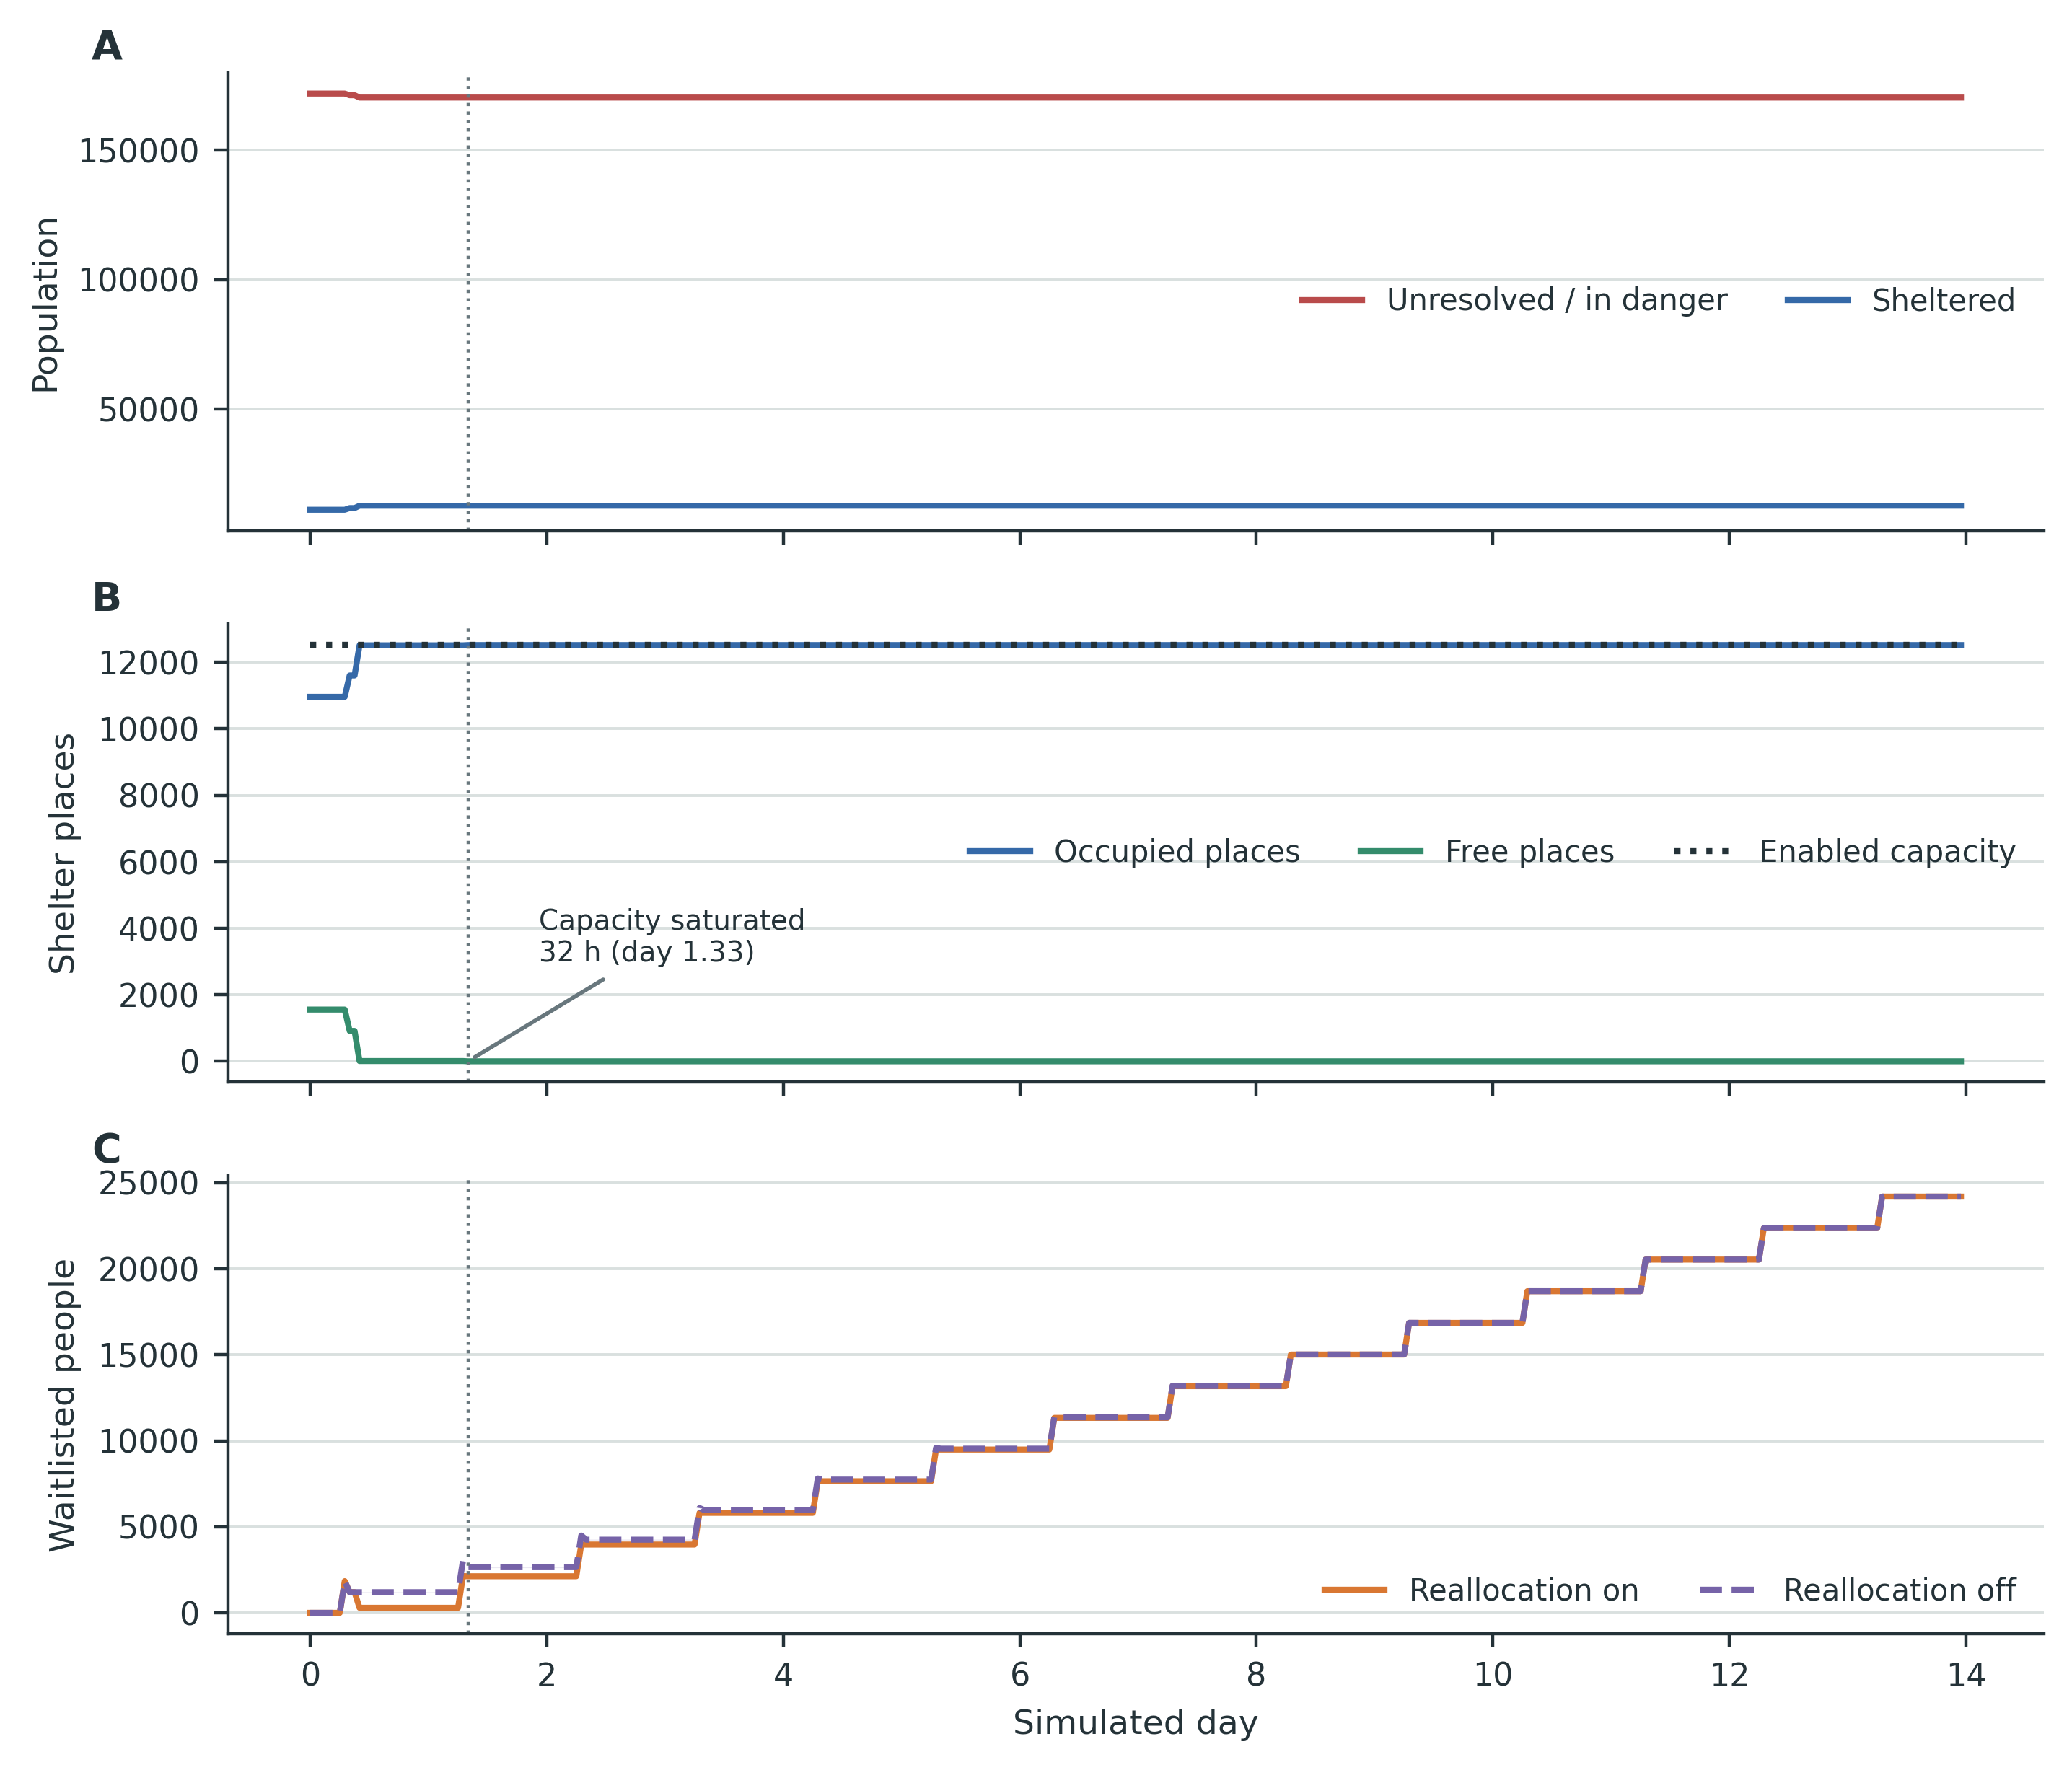
\includegraphics[width=\linewidth]{fig/res-event-disruptions/shelter_reference_dynamics.png}
    \caption{Temporal evolution of the reference shelter experiment over 14 simulated days. Lines show hourly means over five simulation runs. (a) Sheltered and unresolved exposed population with reallocation enabled. (b) Occupied places, free places, and enabled shelter capacity. (c) Total waitlist with reallocation enabled and disabled. The vertical dotted line marks exhaustion of the reference capacity after 32 simulated hours.}
    \label{fig:shelter_reference_dynamics}
\end{figure}

%

The reference scenario therefore illustrates that final coverage alone does not fully characterize evacuation performance. Once capacity is exhausted, redistribution cannot increase the number of people accommodated, but it can reduce how long populations remain waiting for admission.
%SO: tinha gostado mais do meu texto, mas depois vi que tinha uma proxima section sobre isso - VALIDAR
%GA: mantive como esta dada as proximas sections
%These results also highlight a limitation of reallocation when total shelter capacity is fixed. Once the available network reaches full occupancy, redistributing unresolved demand can reduce accumulated waiting but cannot increase final protection. In a real emergency response, however, shelter capacity may evolve over time as new facilities are opened or existing facilities are expanded. Within LODUS, such behavior could be represented by an additional plugin that dynamically creates or activates shelter POIs in response to demand, exposure, or capacity conditions. This would enable future experiments to investigate not only how populations are allocated among existing shelters, but also how adaptive changes to the shelter network could improve protection under evolving demand.

This result suggests that, once the existing shelter network becomes capacity constrained, improving population allocation alone is insufficient and additional shelter capacity is required, motivating the capacity analysis presented next.


\subsubsection{Capacity and Evacuation Demand}
\label{sec:shelter_capacity_response}

The next scenarios examine how shelter capacity and the rate at which exposed populations seek accommodation determine final protection and congestion. Figure~\ref{fig:shelter_sensitivity} summarizes these comparisons.

%SO: nào tem a e b na fig
%GA: são as colunas ao invés de subfigures, ajustei a caption
\begin{figure}[ht]
    \centering
    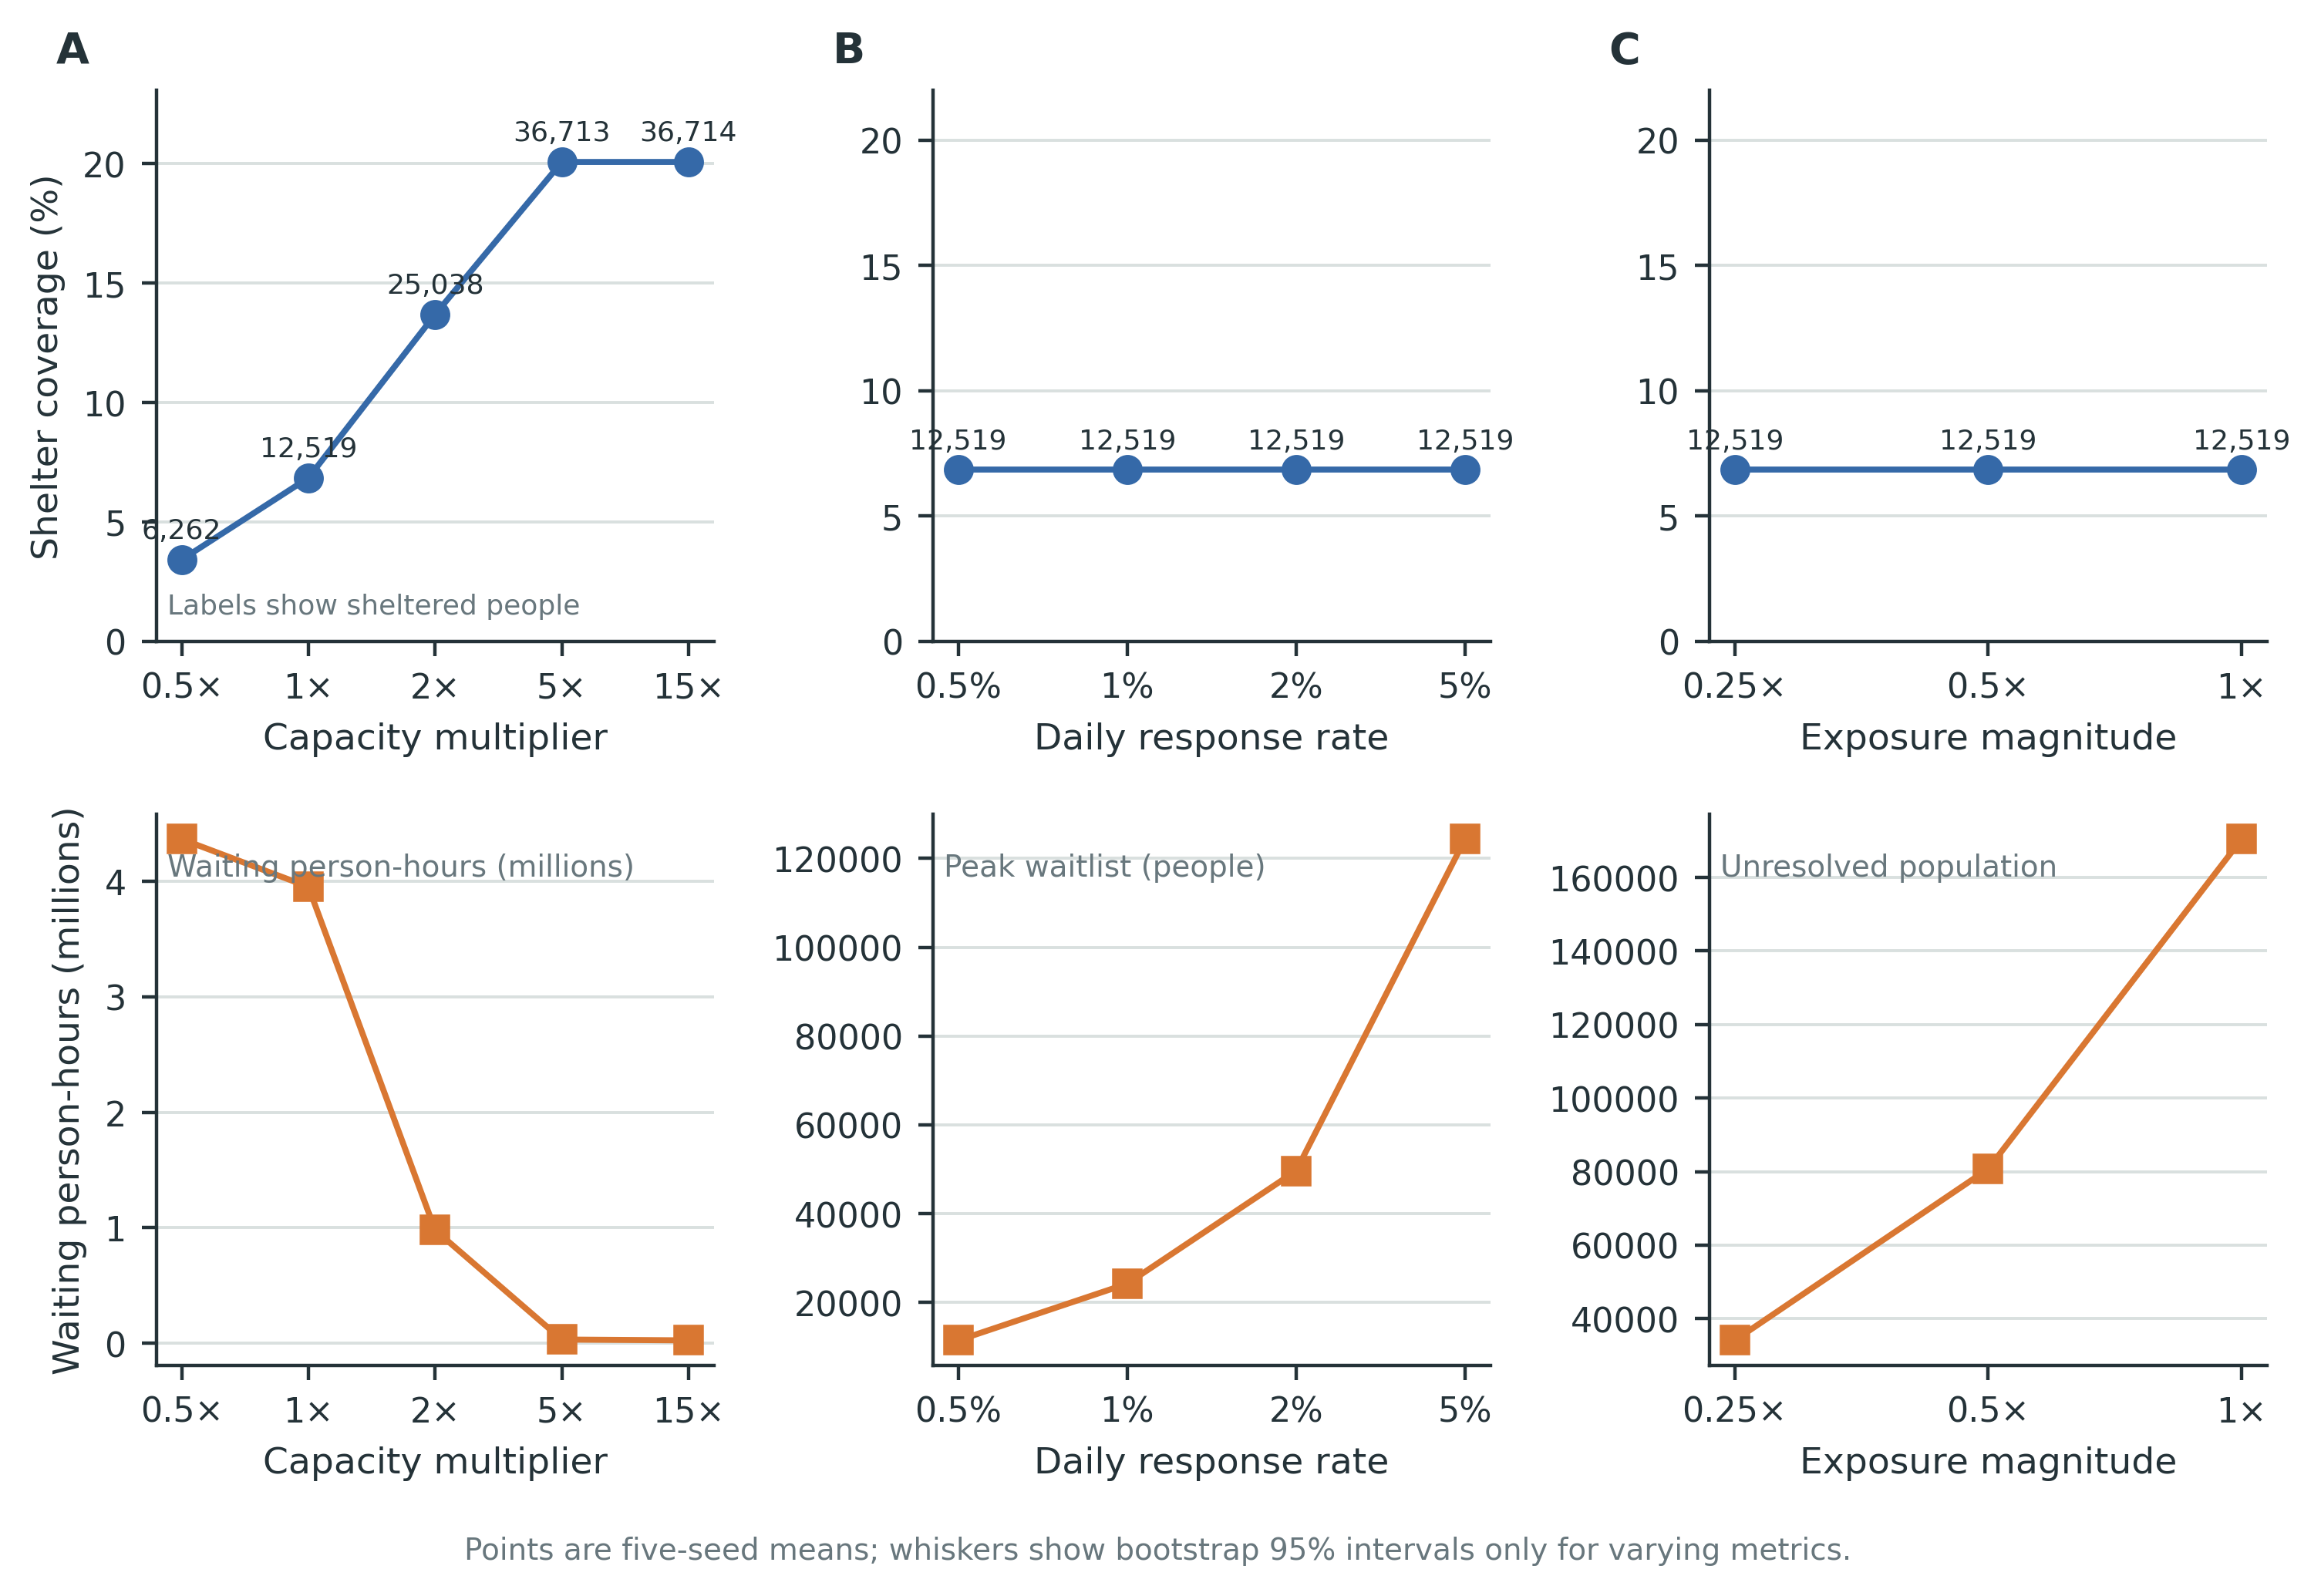
\includegraphics[width=\linewidth]{fig/res-event-disruptions/shelter_sensitivity.png}
    \caption{Shelter outcomes to three scenario parameters: (A) available shelter capacity, (B) daily response rate, and (C) exposure magnitude. The upper row reports final shelter coverage, with labels indicating the number of sheltered people, while the lower row reports the corresponding congestion or unresolved-demand metric: accumulated waiting person-hours for capacity, peak waitlist size for response rate, and unresolved population for exposure magnitude.}
    \label{fig:shelter_sensitivity}
\end{figure}

Increasing shelter capacity substantially improves protection while accommodation remains the principal constraint. Halving the reference capacity reduces final coverage to 3.42\%, whereas doubling it increases coverage to 13.69\%. At five times the reference capacity, coverage reaches approximately 20.07\%.

Increasing capacity further to fifteen times the reference value produces essentially no additional protection during the 14-day simulation. The limiting factor therefore changes as capacity increases. At lower capacity levels, the number of available shelter places limits the population that can be accommodated. Once sufficient capacity exists, the 1\%-per-day response rate and finite simulation duration determine how many exposed people reach shelters before the experiment ends.

Increasing capacity also substantially reduces congestion. Accumulated waiting falls from approximately 3.95 million person-hours under the reference capacity to 0.98 million at twice the capacity and approximately 0.03 million at five times the capacity. The peak waitlist follows the same pattern, falling from 24,195 people to 11,676 and approximately 1,843, respectively.

Changing the daily response rate while keeping capacity fixed produces a different outcome. Final coverage remains 6.843\% for all evaluated response rates because even the slowest condition eventually fills the available shelter network. Higher response rates instead cause this fixed capacity to be consumed earlier and substantially increase queue formation.

At a 0.5\% daily response rate, the peak waitlist is approximately 11,400 people and accumulated waiting is 1.75 million person-hours. At 2\%, these values increase to approximately 49,600 people and 8.36 million person-hours. At 5\%, the peak waitlist exceeds 124,000 people and accumulated waiting reaches approximately 21.4 million person-hours.
Thus, faster evacuation demand does not necessarily result in greater protection. When accommodation remains fixed, it primarily changes how quickly the available places are consumed and how much unresolved demand accumulates around the shelter network.

Exposure scaling provides a complementary demand-side result. Reducing the exposed population does not change the final sheltered population under the reference capacity: all three exposure conditions eventually occupy the same 12,519 places. Lower exposure nevertheless reduces unresolved demand and accumulated waiting. This reinforces the same general relationship between demand and available accommodation without introducing a different limiting mechanism.

Together, these scenarios identify two distinct operating conditions. When shelter space is scarce relative to demand, capacity determines final protection and response speed mainly affects congestion. When capacity becomes sufficiently large, the rate at which exposed populations seek shelter and the duration of the simulation become the principal limits.


\subsubsection{Shelter Failures and Reallocation}
\label{sec:shelter_failures}

The final scenarios examine the effect of losing part of the shelter network. Two disruption conditions are retained. The first disables the single largest shelter, removing 495 places. The second disables the 11 highest-capacity shelters, corresponding to approximately 10\% of the shelter network and removing a combined 3,967 places.

Table~\ref{tbl:shelter_failures} summarizes their effect on final protection with reallocation enabled.

\begin{table}[ht]
\centering
\footnotesize
\caption{Mean shelter outcomes under facility failures over five simulation runs with waitlist reallocation enabled.}
\label{tbl:shelter_failures}
\begin{tabular}{@{}lrrr@{}}
\toprule
\textbf{Condition} &
\shortstack{\textbf{Coverage}\\\textbf{(\%)}} &
\textbf{Unresolved} &
\shortstack{\textbf{Capacity}\\\textbf{removed}} \\
\midrule
No shelter failure
    & 6.843 & 170,417 & --- \\
Largest shelter disabled
    & 6.573 & 170,912 & 495 \\
Top 10\% Highest-capacity shelters disabled
    & 4.675 & 174,384 & 3,967 \\
\bottomrule
\end{tabular}
\end{table}

Disabling the largest shelter reduces coverage from 6.843\% to 6.573\%. Disabling the 11 highest-capacity shelters has a substantially larger effect, reducing coverage to 4.675\%. The difference reflects the amount of accommodation removed from the network: the second condition removes approximately eight times as many places as the failure of the largest individual shelter.

Reallocation cannot restore this lost capacity, but it can reduce congestion among the facilities that remain available. Compared with the corresponding failure scenarios without reallocation, accumulated waiting decreases by approximately 47,000 person-hours after the largest-shelter failure and by 35,000 person-hours after the high-capacity-shelter failures.

\begin{comment}
    
\begin{figure}[ht]
    \centering
    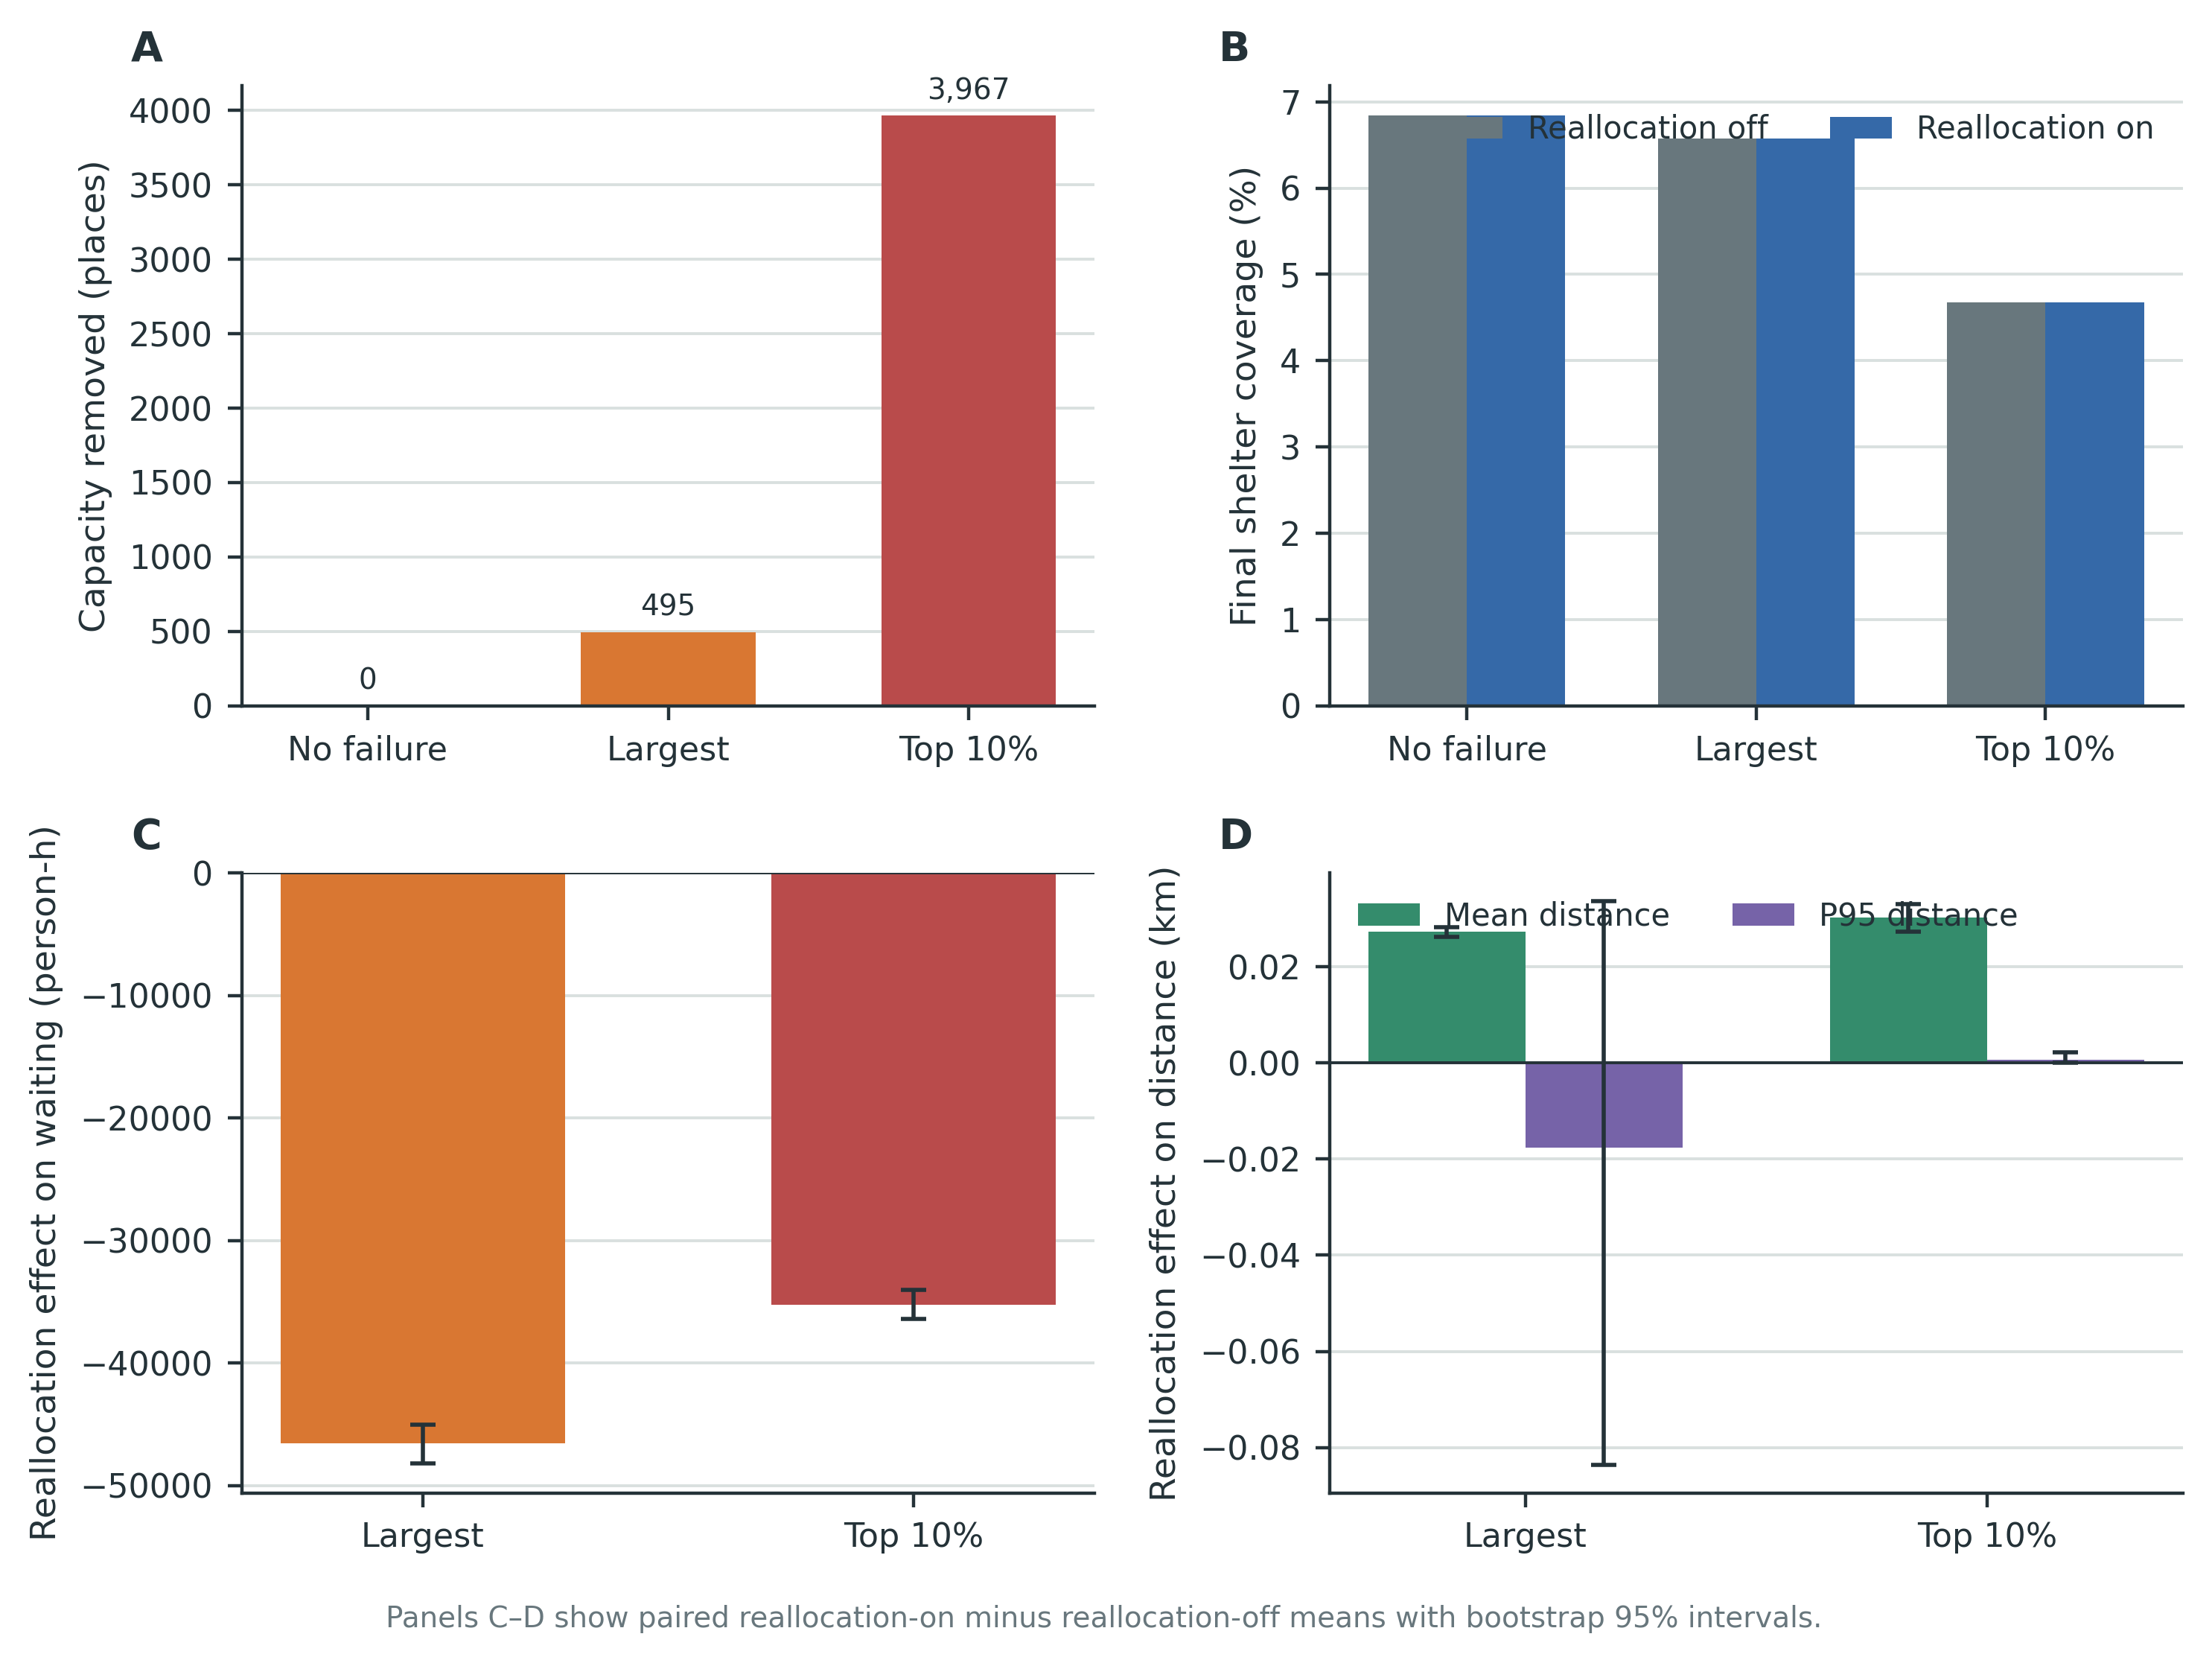
\includegraphics[width=\linewidth]{fig/res-event-disruptions/shelter_failure_robustness.png}
    \caption{Effect of shelter failures and waitlist reallocation on evacuation outcomes. The figure compares the loss of shelter capacity and final coverage under each failure condition and the corresponding reduction in accumulated waiting when reallocation is enabled.}
    \label{fig:shelter_failure_robustness}
\end{figure}
\end{comment}

The failure scenarios reinforce the distinction between accommodation and redistribution. Removing shelter capacity directly reduces the maximum population that can be protected. Reallocation can make better use of the facilities that remain available and reduce waiting, but it cannot recreate the lost accommodation.

Overall, the shelter experiments show that evacuation outcomes depend on the interaction between demand and available service capacity. Under the reference conditions, shelter capacity is exhausted early, limiting final protection while continued evacuation requests generate unresolved demand and congestion. Increasing capacity improves protection until the response rate and simulation horizon become limiting, whereas increasing response speed alone mainly accelerates queue formation. Facility failures further reduce the available protection, while reallocation mitigates waiting without replacing lost capacity. These results demonstrate how exceptional mobility toward a constrained service network differs from the gathering demand examined in the large-scale-event scenarios.





\subsection{Main Findings}
\label{sec:exceptional_disruption_findings}

The experiments in this section examine different ways in which population mobility departs from the normal-life conditions established in the preceding section. Large-scale events introduce additional demand while preserving the availability of the environment, flooding removes some of the origins and destinations required by recurring mobility, and shelter evacuation introduces new movement toward a capacity-constrained service network. Together, these scenarios show that temporary changes in demand and location availability can produce substantially different mobility outcomes even when they operate over the same underlying population and environment representations.

The large-scale-event experiments show that exceptional gathering demand affects both the volume and spatial distribution of movement. Events requesting the same population quantity produce similar aggregate increases when evaluated individually, while their different locations result in distinct displacement-distance distributions. When several events occur simultaneously, their effects are not additive because successive requests operate on a shared and evolving population distribution. Event timing is also relevant: distributing the same four event requests over the day produces more displacement than concentrating them at a single simulation step.

The flood experiments demonstrate how changes in location availability affect different forms of recurring mobility. Activity demand is affected primarily by unavailable destinations, whereas work and school commutes depend on both their origins and their specific destinations. Allowing unavailable activity destinations to be substituted restores almost all requested visits, but shifts part of the disruption into additional travel and increased demand at alternative locations. The same adaptation does not restore work or school attendance because these destinations are not treated as interchangeable in the evaluated configuration. Thus, maintaining mobility demand may require accepting other costs rather than eliminating the effect of the disruption.

The shelter experiments extend this analysis from disrupted recurring mobility to movement generated directly in response to exposure. Under the reference conditions, the shelter network reaches its available capacity early in the simulation, after which additional evacuation demand primarily contributes to unresolved demand and waiting. Increasing shelter capacity improves protection until the response rate and simulation duration become the limiting factors. Conversely, increasing the rate at which exposed populations seek shelter does not increase final protection when capacity remains fixed and instead accelerates congestion. Reallocation reduces waiting by redistributing demand among available facilities, but it cannot increase protection once all available places are occupied or replace capacity removed by shelter failures.

Overall, the results distinguish several consequences of exceptional conditions that would be obscured by considering population movement alone. Additional demand can compete for the population already engaged in other activities; unavailable locations can suppress movement or require alternative destinations; and protective movement can remain constrained by the capacity and availability of the services toward which the population is directed. These experiments therefore complement the normal-life results by showing how the same population representation can support additional demand, mobility disruption, adaptation, and evacuation while preserving the different constraints associated with each scenario.